\documentclass{amsart}[11pt]
\usepackage[
    doi=false,
    isbn=false,
    sortcites,
    backend=biber,   
    firstinits=true,
    maxbibnames=99,
    ]{biblatex} 
\addbibresource{literature.bib}

\usepackage{amsmath, amssymb, amsthm}
\usepackage{fullpage}
\usepackage{hyperref}
\usepackage{algorithm}
\usepackage{algorithmic}
\usepackage{tikz}
\usepackage{enumitem}
\usetikzlibrary{positioning}
\usetikzlibrary{fit}
\newcommand{\layersep}{2.5cm}

\usepackage{color}

\numberwithin{equation}{section}





\newcommand{\nn}{\mathcal{N}}
\newcommand{\card}{\#}
\newcommand{\realization}{\mathcal{R}}
\newcommand{\interpretation}{\mathcal{I}}
\newcommand{\relu}{\sigma}
\newcommand{\true}{\rm TRUE}
\newcommand{\false}{\rm FALSE} 
\newcommand{\cnf}{\mathcal{C}}  
\newcommand{\ksat}{$k$SAT}
\newcommand{\identity}{\rm id}
\newcommand{\order}{\mathcal{O}}
\newcommand{\cost}{\mathcal{C}}
\newcommand{\bool}{\mathcal{B}}
\newcommand{\worstTime}{T}
\newcommand{\powerset}{\mathcal{P}}
\newcommand{\bV}{\mathbf{V}}
 
\input{mymacros.tex}
\numberwithin{theorem}{section}

\newcommand{\fz}[1]{\textcolor{red}{#1}}
\newcommand{\mf}[1]{\textcolor{blue}{#1}}
 
\title{Computational Math with Neural Networks is Hard}
\author{Michael Feischl and Fabian Zehetgruber}
\date{\today}
\thanks{Funded by the Deutsche Forschungsgemeinschaft (DFG, German Research Foundation) -- Project-ID 258734477 -- SFB 1173, the Austrian Science Fund (FWF)
under the special research program Taming complexity in PDE systems (grant SFB F65) as well as project I6667-N. Funding was received also from the European Research Council (ERC) under the
European Union’s Horizon 2020
research and innovation programme (Grant agreement No. 101125225).}

\begin{document} 

 

\begin{abstract}
We show that under some  widely believed assumptions, there are no higher-order algorithms for basic tasks in computational mathematics such as: Computing integrals with  neural network integrands, computing solutions of a Poisson equation with neural network source term, and computing the matrix-vector product with a neural network encoded matrix.
We show that this is already true for very simple feed-forward networks with at least three hidden layers, bounded weights, bounded realization, and sparse connectivity, even if the algorithms are allowed to access the weights of the network. The fundamental idea behind these results is that it is already very hard to check whether a given neural network represents the zero function. The non-locality of the problems above allow us to reduce the approximation setting to deciding whether the input is zero or not. We demonstrate sharpness of our results by providing fast quadrature algorithms for one-layer networks and giving numerical evidence that quasi-Monte Carlo methods achieve the best possible order of convergence for quadrature with neural networks.
\end{abstract}

\maketitle 

\section{Introduction}
\noindent
Neural networks are excellent surrogates for (high-dimensional) functions and perform at least as good as virtually all currently used
specialized (high-dimensional) approximation methods such as polynomials, rational approximation, sparse-grids, tensor networks, \ldots.
Prominent examples of these qualities are given in, e.g.,~\cite{jentzen_approx,schwab_approx,schwab_approx2,schwab_approx3}. Strong results are also available for more involved applications such as solving partial differential equations~\cite{deep_ritz0,deep_ritz1,ZANG2020109409} and inverse problems~\cite{schwab_inverse,berg_inverse}. This even includes problems that are hard for classical approximation methods, such as high-dimensional problems~\cite{schwab_approx2}, fractals~\cite{fractals} or stochastic processes~\cite{jentzen_approx}.
 
 
Thus, two natural questions arise: First, can we efficiently find those networks (for a recent approach to tackle this question, see~\cite{optimalnn}), and second, if we found them, can we efficiently do computations with them. After all, computing a surrogate is usually done with the intention of using it in another algorithm. In this work, we consider the latter question and derive the following result: Under the widely believed \emph{Strong Exponential Time Hypothesis} (SETH), we show for three fundamental tasks from computational mathematics, that even with full knowledge of the neural network representation  of the surrogate (including the weights), no higher-order algorithms exist for the tasks.  
We give a short overview of these tasks in the following.

\emph{Quadrature: } We particularly see quadrature in the sense
\begin{align*}
\Phi \mapsto \int_{\Omega} \realization_\Phi(x) \, dx 
\end{align*} 
for a neural network $\Phi$, its realization function $\realization_\Phi$, and a given domain $\Omega \subseteq \R^d$ as a fundamental task. 
This algorithm is used as a basic building block in countless algorithms, and even in the training of neural networks itself. E.g., for the training of PINNs~\cite{deepRitz_E2018}, one usually has to approximate an integral type norm in order to evaluate the loss function, for Variational Monte Carlo (see, e.g.,~\cite{vmc,Gerard2022GoldstandardST}) the same is true for a scalar product. 
Similar problems arise also for the  Deep Ritz Method~\cite{deepRitz_E2018}, 
eigenvalue problem solvers~\cite{HAN2020109792},  
and weak adversarial methods (e.g.~\cite{ZANG2020109409}).
All these applications usually require some form of quadrature, which is often done with Monte Carlo methods. Since Monte Carlo suffers from slow convergence rates, the natural question is whether we can do better. Clearly, if the neural network represents a smooth function, we can use classical methods such as Gaussian quadrature or high-dimensional methods such as Quasi Monte-Carlo or Sparse Grid quadrature. However, if this is the case, it might be better to not use a neural network approach at all and consider classical high-dimensional approximation methods that are proven to work and are usually much faster.
Thus, the interesting question is whether there exist higher-order quadrature algorithms that do not impose smoothness on the neural network. We show that this is not the case, at least under the assumption of the SETH. We demonstrate experimentally, that quasi-Monte Carlo methods achieve the best possible order of convergence, even for non-smooth neural network integrands.
 
\emph{Solving PDEs: }A similar question arises in the approximation of PDE solutions. It is well-known that smooth maps can be approximated very well with neural networks, which is the foundation of many operator learning approaches.
We refer to the overview articles~\cite{kovachki2024operatorlearningalgorithmsanalysis, azizzadenesheli2024neuraloperatorsacceleratingscientific} 
and the references therein and to~\cite{neuralops,MarcatiChS24,schwab2023deepoperatornetworkapproximation,Lan2022DeepONets} for expression rate bounds.

However, we show that smoothness is really fundamental here. Even for the much simpler linear problem of computing the solution $u_f$ of $-\Delta u_f=f$ with Dirichlet boundary conditions, we show that no higher-order algorithms exist if the right-hand side is represented by a neural network.
This means that no algorithm can efficiently approximate the map
\begin{align*}
\Phi \mapsto u_\Phi\quad\text{ with } -\Delta u_\Phi = \realization_\Phi \text{ and } u_\Phi =0 \text{ on }\partial\Omega.
\end{align*}
While approximating a solution is not the usual operator learning setup, the fundamental fact that no efficient algorithm can be found to approximate a solution to the PDE also precludes the existence of neural networks that approximate the solution operator (despite that in this simple case the solution operator is only a linear operator).


\emph{Matrix-vector multiplication:} Finally, non-linear representations of high-dimensional objects have gained significant interest particularly in the context of low-rank tensor representations, see, e.g.,~\cite{tt1,tt2}. Here, high-dimensional objects such as PDE solutions~\cite{qtt} or large matrices~\cite{ttmatrix} are encoded in tensor formats. 
While these formats come with very efficient arithmetic, we show that similarly efficient algorithms cannot exist for objects that are encoded with neural networks.  To that end, we consider large matrices as one of the simplest objects  that can be used to store high-dimensional data.
Concretely, we consider matrices $M_\Phi\in \R^{2^d\times 2^d}$ defined by
\begin{align*}
(M_{\Phi})_{ij} := \realization_\Phi(b(i)_1,\ldots,b(i)_d,b(j)_1,\ldots,b(j)_d),
\end{align*}
where $b(i)$ is the binary representation of $i$. We show that even simple matrix-vector products with such matrices cannot be computed with higher-order accuracy.


\subsection{Related Work}
Our results can be seen as an extension and generalization of~\cite{t2p} (and recently also~\cite{grohs2025theorytopracticegapneuralnetworks}), which, among other things, shows that there are no higher-order quadrature algorithms based solely on point evaluation for neural network integrands. We show that even the full knowledge of the weights of the neural network cannot be used to get higher-order accuracy.

The works~\cite{liu2024neuralnetworksintegrable,RIVERA2022114710} explore quadrature methods for neural networks and the work~\cite{adaptivequad} proposes the use of adaptive quadrature methods for neural networks and gives some numerical evidence. We stress that our results cover \emph{all} algorithms, including adaptive ones.

We refer to the works~\cite{nphard,np1,np2} and the references therein for NP-hardness results for the neural network training problem. Roughly speaking, the works show that the training of two layer ReLU networks is already NP hard. While our results also relate neural networks with hardness assumptions from computer science, they are independent of the training of the networks.

\subsection{Open Question}
The negative results of this work leave one very interesting open question: 
\begin{quote}
Is there a \emph{relevant} subset of neural networks for which higher-order algorithms exist?
\end{quote}
The term \emph{relevant} requires more explanation: The neural networks in this subset should be expressive outside the classical smoothness regime for which we already have non-neural network approximation methods. Our results show that this subset cannot be characterized by sparsity (at least if the network has more than two layers), boundedness, or low precision of the weights of the networks, thus ruling out many currently used regularization techniques. Moreover,
we show that networks with only two hidden layers are sufficient to prevent higher-order algorithms.
\subsection{Outline of the paper}
In Section~\ref{sec:assumptions}, we introduce some basic concepts and the SETH that our arguments rely on.
In Section~\ref{sec:quad}, we show that no higher-order quadrature algorithms exist for neural networks. We do the same for approximating the solution of a PDE in Section~\ref{sec:pde} and for matrix-vector products in Section~\ref{sec:mvm}. Section~\ref{sec:extensions} discusses several generalizations of our results and shows that there exist fast algorithms for one-layer networks, thus proving that our results are sharp. Moreover, we show that quasi-Monte Carlo methods achieve the best possible order of convergence at least experimentally.

\subsection{Notation}
We use $\N := \{1, 2, 3, \ldots\}$. By $\boldsymbol{1/2}$, we denote the vector $(1/2, \ldots, 1/2) \in \R^d$. The same principle is used for other bold real numbers like $\boldsymbol{1}$. We use $|\cdot|$ for the Euclidean norm and for the Lebesgue measure depending on the context. By $\norm{\cdot}{2}$, we denote the spectral matrix norm. For matrices $\bW$, we use Matlab notation $\bW_{:,i}$ and $\bW_{i,:}$ to denote columns and rows.

\section{Fundamental assumptions and definitions}\label{sec:assumptions}
We introduce some basic notions from theoretical computer science that are relevant for the arguments and statements in this work.
\subsection{Boolean satisfiability problem (SAT)}
The Boolean satisfiability problem (SAT) is the problem of deciding whether a given Boolean formula is satisfiable. A Boolean formula is a formula in propositional logic that consists of variables that can be either $1$ (TRUE) or $0$ (FALSE) and logical connectives such as $\land$ (AND), $\lor$ (OR), and $\lnot$ (NOT). A formula is satisfiable if there exists an assignment of the variables that makes the formula true. An example of a Boolean formula is
\begin{align*}
    (x_1 \lor (x_2 \land \lnot x_3)) \lor (\lnot x_1 \land x_3).
\end{align*}
This formula is for example satisfied by the assignment $x_1 = 0$, $x_2 = 1$, and $x_3 = 1$. There may be multiple assignments that satisfy the same formula.

For every $d \in \N$ and every Boolean formula $\alpha$ with $d$ variables, we define the interpretation $\interpretation_{\alpha}: \{0, 1\}^d \to \{0, 1\}$ that maps an assignment $x \in \{0, 1\}^d$ to the truth value of $\alpha$ under the assignment $x$. The Boolean satisfiability problem is the problem of deciding whether there exists an assignment $x \in \{0, 1\}^d$ such that $\interpretation_{\alpha}(x) = 1$ for a given formula $\alpha$ with $d$ variables.

A literal is a variable $x$ or the negation of a variable $\lnot x$ and a clause is a disjunction of literals (e.g., $x_1\lor \lnot x_2\lor \ldots \lor x_n$). A formula in conjunctive normal form (CNF) is a conjunction of clauses, e.g.,
\begin{align*}
    (x_1 \lor x_2) \land (\lnot x_1 \lor x_3 \lor x_4) \land (\lnot x_2 \lor \lnot x_3).
\end{align*}
Inspired by the way one would represent such a clause in a computer program, we identify a literal with the tuple $(i,\gamma)$, where $i \in \N$ is the index of the variable and $\gamma \in \{\neg, \identity\}$. A clause $C$ is then a set of literals $C = \{\lambda_1, \ldots, \lambda_m\}$, where $m =\# C \in \N$ is the number of literals in the clause. Consequently, a formula $\alpha$ in CNF is a set of clauses $\alpha = \{C_1, \ldots, C_n\}$, where $n = \#\alpha \in \N$ is the number of clauses in the formula.
We denote the set of all possible CNF formulas by $\SS$ and denote
\begin{align*}
    \SS(n) := \set{\alpha \in \SS }{ \text{all }(i,\gamma)\in C\in \alpha\text{ satisfy } 1\leq i\leq n }.
\end{align*}
Furthermore, we will require the subset $\SS_k(n)$, with at most $k$ literals per clause, i.e.,
\begin{align*}
\SS_k(n) := \set{\alpha \in \SS(n)}{ \text{all }C\in \alpha\text{ satisfy } \#C\leq k}.
\end{align*}
Since every clause $C$ in $\alpha \in \SS_k(n)$ consists of at most $k$ literals, there are $2n$ different literals ($x_i$ and $\lnot x_i$ for $i=1,\ldots,n$) and we can also choose to leave a space blank. Hence, $\alpha$ can have at most $\binom{2n+1}{k}$ clauses.


\begin{remark}
    The Tseytin transformation allows us to convert any Boolean formula into an equisatisfiable formula in CNF with length linear in the length of the original formula, see, e.g.,~\cite{Tseitin1983}
\end{remark}

\subsection{Algorithms, computational complexity and models of computation}\label{sec:algorithms}
    In the following, we will make assumptions about the limits of computation. Therefore, it will be necessary to specify the computational model underlying this assumption.
    We will talk about \emph{algorithms} and implicitly assume that those algorithms can be implemented in a computational model for which the \emph{Strong Exponential Time Hypothesis} (SETH) (see Section~\ref{sec:seth} below) is a reasonable assumption.
    Examples for such models of computation are 
    \begin{enumerate}
        \item[(i)] Deterministic Turing machines
        \item[(ii)] Probabilistic Turing machines
        \item[(iii)] Register machines, in particular the Random-Access Machine (RAM) (possibly with access to random numbers).
    \end{enumerate}
    Since all our algorithms (except those of Section~\ref{sec:mvm}) can be implemented in any Turing complete model, it is clear that (i)--(iii) are valid models. For the algorithms in Section~\ref{sec:mvm}, we necessarily require random numbers and hence only models (ii)--(iii) apply. We refer to~\cite{compmodel} for a discussion of the subtle differences between these models.

    In order to talk about computational complexity of an algorithm $\AA$ that takes an input from a set $\Theta$, we define the runtime of the algorithm as follows: Given a subset $\KK\subseteq \Theta$, we define the worst case runtime as
    \begin{align*}
        \worstTime_{\AA}(\KK) := \sup\set{ t > 0 }{\text{there exists input }\btheta \in \KK\text{ such that the computation of }\AA(\btheta) \text{ requires } t \text{ operations}}.
    \end{align*}
    Note that the notion of \emph{operations} depends on the computational model. For example, if we choose a Turing machine as our model of computation, then \emph{operations} refers to the number of steps that the Turing machine takes to compute the output.

\subsubsection{(Probabilistic) decision and approximation algorithms}\label{sec:probalg} 
A decision algorithm $\BB\colon \Theta \to \{0,1\}$ returns a binary output while an approximation algorithm $\AA\colon \Theta \to \R$ returns a real number.
The algorithms in all statements below are allowed to be probabilistic in the sense that they can make truly random decisions at each step during their execution.
This can be modelled with probabilistic Turing machines, and we refer to~\cite{sipser13} for a much more detailed discussion.
%  When we talk about a (probabilistic) algorithm in this paper, we mean a map $\AA\colon \Theta \to \{0,1\}$ or $\AA\colon \Theta \to \R$, where $\Theta$ is a given set of admissible inputs that are finite strings of symbols in a given alphabet $\Xi$, i.e., $\Theta \subseteq \Xi^{[\N]}:=\set{(\xi_1,\ldots,\xi_n)}{n\in \N,\, \xi_i\in \Xi}$. If the algorithm is probabilistic (or randomized), we mean that the algorithm is allowed to make truly random decisions at each step during its execution.  

% On a formal level, this can be modelled with concept of a probabilistic Turing machine. A deterministic Turing machine reads a symbol from an infinite tape and acts according to its transition function $\delta$. A probabilistic Turing machine, on the other hand, has two transition functions $\delta_1$ and $\delta_2$. Every time it reads a symbol from the tape, it flips an (unfair) coin, and decides whether to apply $\delta_1$ or $\delta_2$ based on this coin flip. 

% Following the corresponding definitions for probabilistic Turing machines, we say that an algorithm $\AA\colon \Theta \to \{0,1\}$ solves a problem in $\order(f(n))$-time with an error probability of $1/3$, if 
% \begin{enumerate}[label=(\roman*)]
%     \item\label{item:probabilistic_time_one} $\AA$ produces an output for all inputs $\btheta \in \Theta$ with  maximum length $n$ in at most $\order(f(n))$ steps, 
%     \item\label{item:probabilistic_time_two} for all inputs $\btheta\in \Theta$, the probability that $\AA(\btheta)\in\{0,1\}$ is the correct solution is at least $2/3$,
%     \item\label{item:probabilistic_time_three} for all inputs $\btheta\notin \Theta $, the probability that $\AA$ accepts $\btheta$ as valid input is at most $1/3$. 
% \end{enumerate}
% All statements in this paper can be transferred to this notion of solution with an error probability. 

Note that algorithms with probabilistic runtime can be stopped after a fixed number of steps and return the result of the last step, thus moving uncertainty about runtime to uncertainty about correctness. Therefore, without loss of generality, we may consider algorithms with 
deterministic runtime.

We consider  probabilistic approximation algorithms of the form $\AA\colon  \Theta \to \R$ that come with a prescribed error tolerance $\eps>0$ and a deterministic non-computable ground truth $\TT\colon \Theta \to \R$.
We say that $\AA$ is a probabilistic algorithm with
\begin{align}\label{eq:correctness}
|\AA(\btheta) - \TT(\btheta)|<\eps
\end{align}
if and only if the algorithm satisfies (i)--(iii):
\begin{enumerate}[label=(\roman*)]
    \item\label{item:probabilistic_time_one} $\AA$ produces an output for all inputs $\btheta \in \Theta$, 
    \item\label{item:probabilistic_time_two} for all inputs $\btheta\in \Theta$, the probability that~\eqref{eq:correctness} holds is at least $2/3$,
    \item\label{item:probabilistic_time_three} for all inputs $\btheta\notin \Theta $, the probability that $\AA$ accepts $\btheta$ as valid input is at most $1/3$. 
\end{enumerate}
This mimics the usual definition for probabilistic decision algorithms $\BB\colon \Theta \to \{0,1\}$, which replaces~(ii) with
\begin{enumerate}
    \item[(ii')] For all inputs $\btheta\in \Theta$, the output of $\BB$ is correct with probability at least $2/3$.
\end{enumerate}
Clearly, any probabilistic algorithm $\AA\colon \Theta\to \R$ with~\eqref{eq:correctness} can be extended to a decision algorithm $\BB$ that decides whether~\eqref{eq:correctness} holds. The algorithm $\BB$ then satisfies (i), (ii'), and (iii).

As is the case with probabilistic Turing machines, Lemma~\ref{lem:cluster} below shows that repeated application of a probabilistic approximation algorithm can be used to increase the probability of success.

We note that deterministic algorithms are a proper subset of probabilistic algorithms, in particular they satisfy (ii),~(ii') and reject invalid input (iii) with certainty. Therefore, we do not explicitly mention the probabilistic nature of algorithms in the following.

\subsection{Exponential time hypothesis (ETH)}\label{sec:seth}
In the following, we state the exponential time hypothesis (ETH) first introduced in~\cite{eth} and the strong exponential time hypothesis (SETH) first introduced in~\cite{seth}. Both conjectures give lower bounds on the time complexity for solving SAT problems.
To that end, we define for $k\in\N$ 
\begin{align}\label{eq:s_k_definition}
    s_k := \inf\set{s > 0 }{\text{exists decision algorithm } \AA\text{ for $k$SAT with }\worstTime_{\AA}(\SS_k(n)) = \order(2^{sn}) \text{ for } n \to \infty},
\end{align}
where we take the infimum over all decision algorithms $\AA$ in the sense of Section~\ref{sec:probalg} that satisfy (i), (ii'), and (iii) and decide whether a formula $\alpha\in\SS_k(n)$ is satisfiable or not. 

The infimum is well-defined since for all $k \in \N$ the brute force search over all assignments solves $k$SAT in time $\order(2^{n})$ for $n \to \infty$. This also shows $s_k \leq 1$ for all $k \in \N$. We know that $s_1 = s_2 = 0$ since $1$SAT and $2$SAT problems can be solved in polynomial time~\cite{2sat}. A very simple probabilistic algorithm for $k$SAT that guarantees $s_k\leq 2(1-1/k)+\eps$ for all $k\in\N$ and all $\eps>0$ is the WalkSat algorithm from~\cite{walkSat}.

The ETH can now be stated as follows: For all $k \geq 3$, we have $s_k > 0$.
The nestedness $\SS_k(n)\subseteq \SS_{k+1}(n)$ shows $s_k\leq s_{k+1}$ and hence the limit $\lim_{k \to \infty} s_k$ exists.
The strong exponential time hypothesis (SETH) is even stronger than the ETH and states:
\begin{assumption}[SETH]\label{ass:SETH}
   The numbers $s_k$ satisfy $\lim_{k \to \infty} s_k = 1$.
\end{assumption}
The SETH and in particular the ETH are widely believed to be true and would imply $P\neq NP$, even though they are still open. However, it is known (see, e.g.,~\cite{IMPAGLIAZZO2001512}), that $s_k>0$ for any $k\in\N$ already implies $s_3>0$. This is the reason why SETH is at least as strong as ETH.

In the following, it will be convenient to restrict the problem to formulae that have only a linear number of clauses with respect to the number of variables. The famous sparsification lemma~\cite[Theorem~1]{IMPAGLIAZZO2001512} allows us to reduce SETH to this case.
The sparsification lemma specifies a constant $C=C(k,\eps)$ for $k\in\N$ and $\eps>0$ that is independent of the number of variables $n$. This constant will be used in the proof of Lemma~\ref{lem:sparsification} below as $\widetilde C_k:= C(k,\min\{s_3/3,1/k\})$. We define the set
\begin{align}\label{eq:tildesat}
 \widetilde\SS_k(n):=\set{\alpha \in \SS_k(n)}{\alpha\text{ has at most }\widetilde C_k n\text{ clauses}}.
\end{align}
For this new problem, we also define
\begin{align*}
    \widetilde s_k := \inf\set{s > 0 }{\text{ there exists a decision algorithm } \AA\text{ for $k$SAT with }\worstTime_{\AA}(\tilde{\SS}_k(n)) = \order(2^{sn}) \text{ for } n \to \infty}.
\end{align*}
Again, we have $\widetilde s_k \leq \widetilde s_{k + 1}$ and $\widetilde s_k \leq 1$. This shows that the limit $\lim_{k \to \infty} \widetilde s_k \leq 1$ exists.

\begin{lemma}\label{lem:sparsification}
    Under SETH, we have $\widetilde s_k>0$ for all $k\geq 3$ and $\lim_{k \to \infty} \widetilde s_k=1$.
\end{lemma}
\begin{proof}
   Let us first note that $\widetilde s_k \leq s_k$ for all $k \in \N$ due to $\widetilde \SS_k(n)\subseteq \SS_k(n)$. If $\lim_{k\to \infty} s_k=0$, then $\lim_{k\to \infty} \widetilde s_k=0$ follows immediately. Hence, we can assume that $s_k > 0$ for all $k \geq 3$, which is anyway a consequence of the SETH.
    
   The sparsification lemma~\cite[Theorem~1]{IMPAGLIAZZO2001512} with $\eps_k=\min\{s_3/3,1/k\}$ guarantees the existence of an algorithm $\BB$ that takes a formula $\alpha\in \SS_k(n)$ and
    outputs a disjunction of formulae $\alpha_1, \ldots, \alpha_m$ with $m \leq 2^{\eps_k n}$ such that $\alpha_j\in\widetilde \SS_k(n)$ for all $j = 1, \ldots, m$ and $\alpha$ is satisfiable if and only if at least one of the $\alpha_j$ is satisfiable. The algorithm $\BB$ runs in time $\order(p(n)2^{\eps_k n})$ for $n \to \infty$ for some polynomial $p$. Since satisfiability of all $\alpha_i$ can be decided by an Algorithm $\AA$ in time $\order(2^{(\widetilde s_k + \eps_k) n})$, we can use $\BB$ to construct an algorithm that decides solvability of $\alpha$ in time
    \begin{align*}
    \order(p(n)2^{\eps_k n} + m  2^{(\widetilde s_k + \eps_k) n}) \leq \order(p(n)2^{\eps_k n} + 2^{\widetilde s_k n + 2\eps_k n}) \leq  \order(2^{(\widetilde s_k + 2\eps_k)n}).
    \end{align*}
    This shows
    \begin{align*}
        \widetilde s_k \geq \widetilde s_3 \geq s_3 - 2\eps_3 \geq s_3 - 2 s_3/3 = s_3/3 > 0 \quad \text{for all } k \geq 3.
    \end{align*}
    Furthermore, $s_k\leq \widetilde s_k + 2\eps_k$ and hence $1 = \lim_{k \to \infty} s_k \leq \lim_{k \to \infty} \widetilde s_k \leq 1$ due to the SETH.
\end{proof}

\subsection{Neural networks}
For any subset $\theta \subseteq \R$ we define the set $\nn(d,w,L,\theta)$ of feed-forward neural networks with $d\in\N$ inputs, maximal width $w\in\N$, and maximal depth $L\in\N$ as the set of tuples
\begin{align*}
    \left(\big(\bW_1,\ldots,\bW_{L'}\big),\big(\bb_1,\ldots,\bb_{L'}\big)\right),
\end{align*}
such that $\bW_i\in \theta^{w_{i}\times w_{i-1}}$ and $\bb_i\in \theta^{w_{i}}$ for all $i=1,\ldots,L'$ with numbers $1\leq w_i\leq w$ for all $i=0,\ldots,L'$  such that $w_0 = d$ and $L'\leq L$. Figure~\ref{fig:cnf_to_nn} below shows an example of a feed-forward neural network with $d=4$ inputs, three hidden layers ($L = 4$), and width ten ($w = 10$).

The realization of such a feed-forward network $\Phi \in \nn(d,w,L,\theta)$ is given iteratively by  $\RR_{\Phi, 0}:= {\identity}_{\R^{w_0}}$,
\begin{align*}
\RR_{\Phi, \ell}(x) = \relu(\bW_{\ell}\RR_{\Phi, \ell-1}(x)+ \bb_{\ell})\quad\text{for all }\ell=1,\ldots,L'-1,
\end{align*}
and $\RR_\Phi(x):=\bW_{L'} \RR_{\Phi, L'-1}(x) + \bb_{L'}$. The activation function $\sigma: \R\to \R$ is applied component wise to input vectors. Examples of activation functions are the rectified linear unit (ReLU) $\relu(x) = \max\{0, x\}$ or the hyperbolic tangent $\sigma(x) = \tanh(x)$. We denote the set of all feedforward neural networks as $\nn$. 


In Appendix~\ref{sec:appendix}, we have collected some well known results that show how operations like addition or composition of neural networks can be performed efficiently, at least in the case of ReLU networks. Throughout this paper we will need the following construction of Lemma~\ref{lem:CNF_to_nn} that shows how to convert a CNF formula into a neural network.



\begin{lemma}\label{lem:CNF_to_nn}
    Suppose $\Psi \in \NN(1, w_r, L_r, \theta_r)$ and $r: \R \to [0, 1]$ is such that $\realization_\Psi(x) = r(x)$ holds for all $x \in \R$. If $\alpha \in \widetilde \SS_k(n)$ for some $n \in \N$, then there exists 
    \begin{align*}
        \Phi_\alpha \in \nn(n, \widetilde C_k n w_r k, 3L_r - 2, \theta_{\rm{CNF}})
    \end{align*}
    such that 
    \begin{align}\label{eq:CNF_to_nn}
        \realization_{\Phi_\alpha}(x) = r\left(\rho + \sum_{C \in \alpha} \left(r\left(\sum_{(i, \gamma) \in C} r\left(\gamma x_i\right)\right) - \rho\right)\right).
    \end{align}
    The set $\theta_{\rm{CNF}}$ is a fixed, finite set of weights that contains $\theta_r$, the numbers $\{-1 ,-\rho, 0, \rho,1\}$ and all numbers that occur due to the construction of $\Phi_\alpha$.
\end{lemma}
\begin{proof}
    It is well-known (see, e.g., Appendix~\ref{sec:appendix} for details) that composition of two neural networks of depths $L_1$ and $L_2$ results in a neural network with depth $L_1+L_2-1$ and the maximum of the two widths. Moreover, computing the sum of $n$ neural networks with widths $w_1,\ldots,w_n$ and the same depths $L$ results in a neural network with width $w_1+\ldots+w_n$ and depth $L$.

    For every clause $C\in \alpha$ and every $(i, \gamma) \in C$, we can construct a neural network $\Phi_{C,i,\gamma} \in \nn(n, w_r, L_r, \theta_{\rm{CNF}})$ such that
    \begin{align*}
        \realization_{\Phi_{C,i,\gamma}}(x) = r(\gamma x_i).
    \end{align*}
    By summing over all $(i, \gamma) \in C$ and subtracting $\rho$ we can construct a neural network $\Phi_C \in \nn(n, w_rk, L_r, \theta_{\rm{CNF}})$ such that
    \begin{align*}
        \realization_{\Phi_C}(x) = \left(\sum_{(i, \gamma) \in C} r(\gamma x_i)\right) - \rho.
    \end{align*}
    Again, by using summation of networks with equal depth, adding a bias in the final layer, and composition, we show the existence of a neural network $\Phi_\alpha \in \nn(n, \widetilde C_k n w_r k, 3L_r - 2, \theta_{\rm{CNF}})$ such that~\eqref{eq:CNF_to_nn} holds. 
\end{proof}

This construction is also illustrated by Algorithms~\ref{alg:clause_to_nn} and~\ref{alg:cnf_to_nn} in Appendix~\ref{sec:appendix} below.


% \begin{figure}[h]
%     \centering
%     \begin{tikzpicture}[shorten >=1pt,->,draw=black!50, node distance=\layersep]
%         \tikzstyle{every pin edge}=[<-,shorten <=1pt]
%         \tikzstyle{neuron}=[circle,fill=black!25,minimum size=17pt,inner sep=0pt]
%         \tikzstyle{input neuron}=[neuron, fill=green!50];
%         \tikzstyle{output neuron}=[neuron, fill=red!50];
%         \tikzstyle{hidden neuron}=[neuron, fill=blue!50];
%         \tikzstyle{annot} = [text width=4em, text centered]

%         % Draw the input layer nodes
%         \foreach \name / \y in {1,...,3}
%             \node[input neuron, pin=left:Input \y] (I-\name) at (0,-\y) {};

%         % Draw the first hidden layer nodes
%         \foreach \name / \y in {1,...,5}
%             \node[hidden neuron] (H1-\name) at (\layersep,-\y+1) {};

%         % Draw the second hidden layer nodes
%         \foreach \name / \y in {1,...,4}
%             \node[hidden neuron] (H2-\name) at (2*\layersep,-\y+0.5) {};

%         % Draw the output layer nodes
%         \foreach \name / \y in {1,...,2}
%             \node[output neuron, pin={[pin edge={->}]right:Output \y}] (O-\name) at (3*\layersep,-\y-0.5) {};

%         % Connect every node in the input layer with every node in the first hidden layer
%         \foreach \source in {1,...,3}
%             \foreach \dest in {1,...,5}
%                 \path (I-\source) edge (H1-\dest);

%         % Connect every node in the first hidden layer with every node in the second hidden layer
%         \foreach \source in {1,...,5}
%             \foreach \dest in {1,...,4}
%                 \path (H1-\source) edge (H2-\dest);

%         % Connect every node in the second hidden layer with every node in the output layer
%         \foreach \source in {1,...,4}
%             \foreach \dest in {1,...,2}
%                 \path (H2-\source) edge (O-\dest);

%         % Annotate the layers
%         \node[annot,above of=I-1, node distance=1cm] (il) {Input layer};
%         \node[annot,above of=H1-1, node distance=1cm] (hl1) {Hidden layer 1};
%         \node[annot,above of=H2-1, node distance=1cm] (hl2) {Hidden layer 2};
%         \node[annot,above of=O-1, node distance=1cm] (ol) {Output layer};
%     \end{tikzpicture}
%     \caption{Feedforward neural network architecture} \label{fig:nn_architecture}
% \end{figure}


\section{Quadrature of neural networks}\label{sec:quad}
In this section, we show that any higher order quadrature algorithm for neural networks implies an efficient algorithm that decides the $k$SAT problem. This contradicts the SETH (Assumption~\ref{ass:SETH}) and hence shows that higher-order quadrature for neural network integrands is hard.

\subsection{SAT problems, numerical quadrature and neural networks}
We show in an abstract setting that we can decide whether a formula is satisfiable by integrating a particular function associated with the formula.

\begin{lemma}\label{lem:quad_to_sat}
    For $d \in \N$, let $\mu$ be probability measure on $\Omega\subseteq \R^d$. Suppose $\kappa, \rho, \nu > 0$ are real numbers such that $\kappa < \nu \rho$ and for every Boolean formula $\alpha$, we have an associated integrable function $F_\alpha: \Omega \to [0, \infty)$ with the properties:
    \begin{enumerate}[label=(\roman*)]
        \item\label{item:function_is_zero} If $\alpha$ is not satisfiable, $F_\alpha(x) \leq \kappa$ for all $x \in \Omega$.
        \item\label{item:function_is_positive} If $\alpha$ is satisfiable, there exists a set $Q_\alpha \subseteq \Omega$ with $\mu(Q_\alpha) \geq \nu$ such that $F_\alpha(x) \geq \rho$ for all $x \in Q_\alpha$.
    \end{enumerate}
    Then, $\alpha$ is satisfiable if and only if $\int_{\Omega} F_\alpha \, d\mu \geq \nu \rho$.
\end{lemma}
\begin{proof}
    If $\alpha$ is not satisfiable, then~\ref{item:function_is_zero} implies
    \begin{align*}
        \int_{\Omega} F_\alpha \, d\mu \leq \kappa < \nu \rho.
    \end{align*}
    On the other hand, if $\alpha$ is satisfiable, then~\ref{item:function_is_positive} implies
    \begin{align*}
        \int_{\Omega} F_\alpha \, d\mu \geq \int_{Q_\alpha} F_\alpha \, d\mu \geq \mu(Q_\alpha) \rho \geq \nu \rho.
    \end{align*}
    This concludes the proof.
\end{proof}

Numerical quadrature is already sufficient to decide whether a formula is satisfiable. 

\begin{lemma}\label{lem:quad_to_sat_algorithm}
    In addition to the assumptions of Lemma~\ref{lem:quad_to_sat}, we assume that we have an approximation algorithm $\AA(\alpha)$ satisfying 
    \begin{align}\label{eq:quad}
        \left|\AA(\alpha) - \int_{\Omega} F_\alpha \, d\mu\right| < \frac{\nu\rho - \kappa}{2}
    \end{align}
    for a formula $\alpha$.
    Then, the algorithm that checks $\AA(\alpha) > \frac{\nu \rho + \kappa}{2}$ decides the satisfiability of $\alpha$.
\end{lemma}
\begin{proof}
    The output of $\AA$ satisfies~\eqref{eq:quad}. In this case, if $\alpha$ is not satisfiable, then $|F_\alpha(x)| \leq \kappa$ for all $x \in \Omega$. This implies
    \begin{align*}
        \AA(\alpha) &\leq \left|\int_{\Omega} F_\alpha \, d\mu - \AA(\alpha)\right| + \left|\int_{\Omega} F_\alpha \, d\mu \right| < \frac{\nu \rho - \kappa}{2} + \kappa = \frac{\nu \rho + \kappa}{2}.
    \end{align*}
    On the other hand, if $\alpha$ is satisfiable, then
    \begin{align*}
        \AA(\alpha) &\geq \int_{\Omega} F_\alpha \, d\mu - \left|\int_{\Omega} F_\alpha \, d\mu - \AA(\alpha)\right| >  \int_{\Omega} F_\alpha \, d\mu - \frac{\nu \rho - \kappa}{2} \geq \nu \rho - \frac{\nu \rho - \kappa}{2} = \frac{\nu \rho + \kappa}{2}.
    \end{align*}
    This concludes the proof.
\end{proof}


In the following, we will set $F_\alpha(x)=\realization_{\Phi_\alpha}(x)$. We require the following simple observation.
\begin{lemma}\label{lem:not_satisfiable}
    Given $\alpha\in\SS(n)$ that is not satisfiable, for every $x \in [0, 1]^n$ there exists a clause $C_x \in \alpha$ such that $\gamma x_i \leq 1/2$ holds for all $(i, \gamma) \in C_x$.
\end{lemma}
\begin{proof}
    Given $x \in [0, 1]^n$, let $z(x) \in \{0, 1\}^n$ be a point with minimal distance to $x$. If $\alpha$ is not satisfiable then there exists a clause $C_x \in \alpha$ such that $z(x)$ does not satisfy $C_x$, i.e., $\interpretation_{\{C_x\}}(z(x))=0$. This implies that for all literals $(i, \gamma) \in C_x$, we have $\gamma z(x)_i = 0$. Since $z(x)$ in $\{0, 1\}^n$ has minimal distance to $x$ we have $|x_i - z(x)_i| \leq 1/2$ for all $i \in \{1, \ldots, n\}$. Therefore,
    \begin{align*}
        \gamma x_i \leq \gamma z(x)_i + |\gamma x_i - \gamma z(x)_i| = |x_i - z(x)_i| \leq 1/2
    \end{align*}
    holds for all $(i, \gamma) \in C_x$.
\end{proof}

The following proposition states simple sufficient conditions for $r$ that allow us to decide whether a formula is satisfiable via integration of the associated function $F_\alpha$.

\begin{proposition}\label{prop:relu_sufficient_properties_of_rd}
    Let $d, k, n \in \N$ with $n \leq d$ and $0 < \delta < 1/2$. Suppose $\Psi \in \nn(1, w_r, L_r, \theta_r)$ and $r: \R \to [0, 1]$ is a continuous function such that\\
    \begin{minipage}{0.6\textwidth}
    \begin{enumerate}
        \item[(i)] $r(x) = 0$ holds for all $-\infty < x \leq 1/2$,
        \item[(ii)] $r(x) = 1$ holds for all $1 - \delta \leq x < \infty$,
        \item[(iii)] $\realization_\Psi(x) = r(x)$ for all $x \in \R$.
    \end{enumerate}
\end{minipage}
\begin{minipage}{0.35\textwidth}
    \includegraphics[width=\textwidth]{rfct.eps}
\end{minipage}\\
    For every formula $\alpha \in \widetilde \SS_k(n)$ we define $\Phi_\alpha$ as in Lemma~\ref{lem:CNF_to_nn} with $\rho = 1$. Then, $F_\alpha: [0, 1]^d \to [0, 1]$, $F_\alpha(x) = \realization_{\Phi_\alpha}(x_1, \ldots, x_n)$ satisfies the assumptions of Lemma~\ref{lem:quad_to_sat} with $\kappa=0$, $\rho=1$, $\nu = \delta^n$, and $\Omega=[0,1]^d$. For satisfiable $\alpha$, the set $Q_\alpha$ can be chosen as
    \begin{align}\label{eq:Qalpha}
        Q_\alpha = \left\{x \in [0, 1]^d \, \middle| \, \max_{i \in \{1, \ldots, n\}} |z_{i} - x_i| \leq \delta\right\}
    \end{align}
    for any $z \in \{0,1\}^d$ with $\interpretation_\alpha(z_1, \ldots, z_n) = 1$.
\end{proposition}
\begin{proof}
    If $\alpha$ is not satisfiable, then Lemma~\ref{lem:not_satisfiable} shows that for every $x \in [0, 1]^d$ there exists a clause $C_x \in \alpha$ such that $\gamma x_i \leq 1/2$ holds for all $(i, \gamma) \in C_x$. This implies $\sum_{(i, \gamma) \in C_x} r(\gamma x_i) = 0$ and therefore $r\left(\sum_{(i, \gamma) \in C_x} r(\gamma x_i)\right) = 0$. From this we deduce
    \begin{align*}
        \sum_{C \in \alpha} r\left(\sum_{(i, \gamma) \in C} r\left(\gamma x_i\right) \right) = 0
    \end{align*}
    and consequently $F_\alpha(x) = 0$ for all $x \in [0, 1]^d$.

    If $\alpha$ is satisfiable, then there exists $z \in \{0, 1\}^d$ such that $\interpretation_{\alpha}(z) = 1$. In particular, $(z_1, \ldots, z_n)$ satisfies all clauses $C\in\alpha$. For any clause $C\in \alpha$, there exists $(j, \gamma) \in C$ such that $\gamma z_{j} = 1$. The set $Q_\alpha$ given by~\eqref{eq:Qalpha} satisfies $|Q_\alpha| = \delta^n$, where $|\cdot|$ is the Lebesgue measure on $[0, 1]^d$. For all $x \in Q_\alpha$ we have
    \begin{align*}
        \gamma x_j = \gamma z_{j} + \gamma x_j - \gamma z_{j} \geq 1 - |x_j - z_{j}| \geq 1 - \delta.
    \end{align*}
    This implies $\sum_{(i, \gamma) \in C} r(\gamma x_i) \geq 1$ and therefore $r\left(\sum_{(i, \gamma) \in C} r\left(\gamma x_i\right) \right) = 1$. From this we deduce
    \begin{align*}
        \sum_{C \in \alpha} \left(r\left(\sum_{(i, \gamma) \in C}  r\left(\gamma x_i\right) \right) - 1\right) \geq 0
    \end{align*}
    and consequently $F_\alpha(x) = 1$ for all $x \in Q_\alpha$. 
\end{proof}


It remains to show that a suitable function $r$ can be constructed with neural networks. We demonstrate this for ReLU activation.
\begin{lemma}\label{lem:r_with_relu}
    Let $\tau > 0$ and $\sigma: \R \to \R$ be the ReLU activation function $\sigma(x) = \max\{0, x\}$. With 
    \begin{align*}
        \theta_r = \left\{- (2\tau)^{-1}, -1, 0, -(1 + 2\tau), 2, (2\tau)^{-1}\right\}
    \end{align*}
    there exists a neural network $\Psi \in \nn(1, 2, 2, \theta_r)$ and a  function $r: \R \to [0, 1]$ such that
    \begin{align*}
        \realization_\Psi(x) = r(x) = (2\tau)^{-1} \sigma\left(2x - 1\right) - (2\tau)^{-1} \sigma\left(2x - \left(1 + 2\tau\right) \right).
    \end{align*}
    Given $0 < \delta < 1/2$, the properties of Proposition~\ref{prop:relu_sufficient_properties_of_rd} are satisfied with $\tau = 1/2 - \delta$.
\end{lemma}
\begin{proof}
    % We illustrate in the picture what the neural network we are constructing looks like.
    % \begin{center}
    %     \begin{tikzpicture}[shorten >=1pt,->,draw=black!50, node distance=2cm]
    %         \tikzstyle{neuron}=[circle,minimum size=17pt,inner sep=0pt]
    %         \tikzstyle{input neuron}=[neuron, draw=black, circle];
    %         \tikzstyle{output neuron}=[neuron,  draw=black, circle];
    %         \tikzstyle{hidden neuron}=[neuron, draw=black, rectangle];
    %         \tikzstyle{annot} = [text width=4em, text centered]
            
    %         % Draw the input layer node
    %         \node[input neuron] (I) at (0,0) {$x$};
        
    %         % Draw the hidden layer nodes
    %         \node[hidden neuron] (H1) at (2,0.5) {$-1$};
    %         \node[hidden neuron] (H2) at (2,-0.5) {$-(1 + 2\tau)$};
        
    %         % Draw the output layer node
    %         \node[output neuron] (O) at (5,0) {$0$};
        
    %         % Connect the input layer to the hidden layer
    %         \path (I) edge node[above] {$2$} (H1);
    %         \path (I) edge node[below] {$2$} (H2);
        
    %         % Connect the hidden layer to the output layer
    %         \path (H1) edge node[above right] {$(2\tau)^{-1}$} (O);
    %         \path (H2) edge node[below] {$-(2\tau)^{-1}$} (O);
        
    %         % Annotate the layers
    %         \node[annot,above of=H1, node distance=1cm] (hl) {Hidden layer};
    %         \node[annot,left of=hl] {Input layer};
    %         \node[annot,above of=O, node distance=1.5cm] {Output layer};
    %     \end{tikzpicture}
    %     \end{center}

        For $x \leq 1/2$ we have $r(x) = 0$. For $1/2 < x \leq 1/2 + \tau$ we have $ r(x) = \tau^{-1} \left(x - \frac{1}{2}\right) $. Finally, for $x > 1/2 + \tau$ we have 
        \begin{align*}
            r(x) = (2\tau)^{-1} \left(2x - 1\right) - (2\tau)^{-1} \left(2x - \left(1 + 2\tau\right) \right) = 1.
        \end{align*}
        This shows that $r$ satisfies the properties of Proposition~\ref{prop:relu_sufficient_properties_of_rd} with $\tau = 1/2 - \delta$.
\end{proof}

\begin{figure}[h]
    \centering
    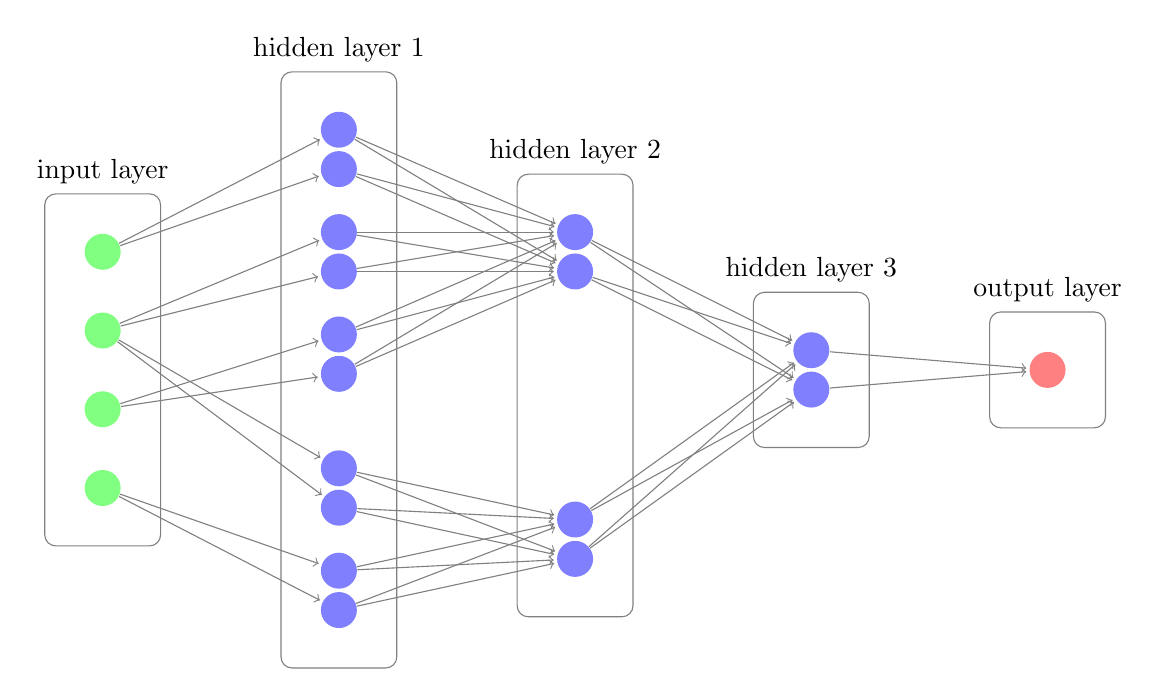
\begin{tikzpicture}[shorten >=1pt,->,draw=black!50, node distance=\layersep]
        \tikzstyle{every pin edge}=[<-,shorten <=1pt]
        \tikzstyle{neuron}=[circle,fill=black!25,minimum size=13pt,inner sep=0pt]
        \tikzstyle{input neuron}=[neuron, fill=green!50];
        \tikzstyle{output neuron}=[neuron, fill=red!50];
        \tikzstyle{hidden neuron}=[neuron, fill=blue!50];
        \tikzstyle{annot} = [text width=4em, text centered]
        % Parameters
        \def\clauseSep{4.3}
        \def\pairSep{1.3}
        \def\inPairSep{0.5}
        \def\layersep{3.0}

        % Input layer (now 4 variables)
        \foreach \name / \y in {1,...,4}
            \node[input neuron] (I-\name) at (0,-\y) {};

        % Calculate centers
        \def\inputCenter{-2.5}
        \pgfmathsetmacro{\hiddenTop}{0 + 0.5*\inPairSep}
        \pgfmathsetmacro{\hiddenBottom}{-\clauseSep -1*\pairSep -0.5*\inPairSep} % 2 pairs in 2nd clause
        \pgfmathsetmacro{\hiddenCenter}{0.5*(\hiddenTop+\hiddenBottom)}
        \pgfmathsetmacro{\hiddenShift}{\inputCenter-\hiddenCenter}

        % First hidden layer: pairs for each literal in each clause
        % Clause 1: 3 literals (x1, x2, x3)
        \foreach \pair [count=\p from 0] in {1,2,3} {
            \pgfmathsetmacro{\y}{-0*\clauseSep -\p*\pairSep}
            \node[hidden neuron] (H1-1-\pair-1) at (\layersep, {\y + 0.5*\inPairSep + \hiddenShift}) {};
            \node[hidden neuron] (H1-1-\pair-2) at (\layersep, {\y - 0.5*\inPairSep + \hiddenShift}) {};
        }
        % Clause 2: 2 literals (x2, x4)
        \foreach \pair [count=\p from 0] in {1,2} {
            \pgfmathsetmacro{\y}{-1*\clauseSep -\p*\pairSep}
            \node[hidden neuron] (H1-2-\pair-1) at (\layersep, {\y + 0.5*\inPairSep + \hiddenShift}) {};
            \node[hidden neuron] (H1-2-\pair-2) at (\layersep, {\y - 0.5*\inPairSep + \hiddenShift}) {};
        }

        % Second hidden layer: pair at center of each clause
        \foreach \clause/\numPairs in {1/3,2/2} {
            \pgfmathsetmacro{\clauseTop}{-(\clause-1)*\clauseSep + 0.5*\inPairSep + \hiddenShift}
            \pgfmathsetmacro{\clauseBottom}{-(\clause-1)*\clauseSep -(\numPairs-1)*\pairSep -0.5*\inPairSep + \hiddenShift}
            \pgfmathsetmacro{\clauseCenter}{0.5*(\clauseTop+\clauseBottom)}
            \node[hidden neuron] (H2-\clause-1) at (2*\layersep, {\clauseCenter + 0.25}) {};
            \node[hidden neuron] (H2-\clause-2) at (2*\layersep, {\clauseCenter - 0.25}) {};
        }

        % Third hidden layer: pair at center of all hidden nodes
        \pgfmathsetmacro{\layerCenter}{\hiddenCenter+\hiddenShift}
        \node[hidden neuron] (H3-1) at (3*\layersep, {\layerCenter + 0.25}) {};
        \node[hidden neuron] (H3-2) at (3*\layersep, {\layerCenter - 0.25}) {};

        % Output layer: single node at center
        \node[output neuron] (O) at (4*\layersep, {\layerCenter}) {};

        % Connect input to first hidden layer: each pair to its variable
        % Clause 1: literals x1, x2, x3
        \foreach \pair/\var in {1/1,2/2,3/3}
            \foreach \j in {1,2}
                \draw (I-\var) -- (H1-1-\pair-\j);
        % Clause 2: literals x2, x4
        \foreach \pair/\var in {1/2,2/4}
            \foreach \j in {1,2}
                \draw (I-\var) -- (H1-2-\pair-\j);

        % Connect first hidden to second hidden layer
        \foreach \clause/\numPairs in {1/3,2/2}
            \foreach \pair in {1,...,\numPairs}
                \foreach \j in {1,2}
                    \foreach \k in {1,2}
                        \draw (H1-\clause-\pair-\j) -- (H2-\clause-\k);

        % Connect second to third hidden layer
        \foreach \clause in {1,2}
            \foreach \j in {1,2}
                \foreach \k in {1,2}
                    \draw (H2-\clause-\j) -- (H3-\k);

        % Connect third hidden to output
        \foreach \j in {1,2}
            \draw (H3-\j) -- (O);

        % Optionally, annotate layers
        % \node[annot, text width=100pt, above of=I-1, node distance=0.7cm] (il) {input layer};
        % %\node[annot, text width=100pt,above of=H1-1-1-1, node distance=0.5cm] (hl1) {hidden layer 1};
        % \node[annot, text width=100pt,above of=H2-1-1, node distance=0.6cm] (hl2) {hidden layer 2};
        % \node[annot, text width=100pt,above of=H3-1, node distance=0.7cm] (hl3) {hidden layer 3};
        % \node[annot, text width=100pt,above of=O, node distance=0.5cm] (ol) {output layer};
        \node[draw, rounded corners, fit=(I-1)(I-2)(I-3)(I-4), inner sep=5mm, label=above:{input layer}] {};
        \node[draw, rounded corners, fit=(H1-1-1-1)(H1-1-3-2)(H1-2-1-1)(H1-2-2-2), inner sep=5mm, label=above:{hidden layer 1}] {};
        \node[draw, rounded corners, fit=(H2-1-1)(H2-1-2)(H2-2-1)(H2-2-2), inner sep=5mm, label=above:{hidden layer 2}] {};
        \node[draw, rounded corners, fit=(H3-1)(H3-2), inner sep=5mm, label=above:{hidden layer 3}] {};
        \node[draw, rounded corners, fit=(O), inner sep=5mm, label=above:{output layer}] {};
    \end{tikzpicture}
    \caption{The connectivity graph of $\Phi_\alpha$ from Lemma~\ref{lem:CNF_to_nn} for formulas $\alpha$ of the form $(\gamma_1 x_1 \lor \gamma_2 x_2 \lor \gamma_3 x_3) \land (\gamma_4 x_2 \lor \gamma_5 x_4)$ with $\gamma_i\in \{{\rm id},\lnot\}$.} \label{fig:cnf_to_nn}
\end{figure}

This particular construction of $r$ allows us to give precise sparsity bounds for the weight matrices of $\Phi_\alpha$ in Lemma~\ref{lem:CNF_to_nn}.
Note that we can obtain similar sparsity bounds for all networks used below in Theorems~\ref{thm:hardness_hypercube1}--\ref{thm:hardness_hypercube2},~\ref{thm:hardness_ball_low_precision}--\ref{thm:hardness_general},~\ref{thm:hardness_pde},~\ref{thm:hardness_mvm}.
\begin{proposition}\label{prop:sparsity}
With $\Psi$ from Lemma~\ref{lem:r_with_relu}, each weight matrix $\bW_i$ of $\Phi_\alpha$ from Lemma~\ref{lem:CNF_to_nn} has at most $4k \widetilde C_k n$ non-zero entries.
\end{proposition}
\begin{proof}
    We refer to Figure~\ref{fig:cnf_to_nn} for a sketch of the connectivity graph for some generic $\Phi_\alpha$.
By construction of $\Phi_\alpha$ in Lemma~\ref{lem:CNF_to_nn}, we see that the first layer is a parallelization of $\Psi$ from Lemma~\ref{lem:r_with_relu} for all literals $(i, \gamma) \in C$. Since each weight matrix of $\Psi$ has at most two non-zero entries, the number of non-zero entries in the first weight matrix $\bW_1$ of $\Phi_\alpha$ is bounded by $2k \widetilde{C}_k n$. 

The second weight matrix $\bW_2$ is a block diagonal matrix with at most $\card \alpha = \widetilde C_k n$ blocks, where each block corresponds to a clause $C\in\alpha$. Each block is of size $2 \times 2k$ and has at most $4k$ non-zero entries. Thus, the second weight matrix $\bW_2$ has at most $4k \widetilde C_k n$ non-zero entries.
The matrix $\bW_3$ has shape $2 \times 2 \widetilde C_k n$ with at most $4\widetilde C_k n$ non-zero entries. 
Finally, the matrix $\bW_4$ is a $1 \times 2$ matrix with at most $2$ non-zero entries.
\end{proof}

\subsection{Quadrature on the hypercube}\label{sec:quadrature_hypercube}
Given $n, d \in \N$ and a neural network $\Phi \in \nn(d, w, L, \theta)$ we would like to find algorithms $\AA$ such that $\AA(\Phi)$ approximates the integral
\begin{align}\label{eq:hypercub_ground_truth}
    \int_{[0,1]^{d}} \RR_\Phi(x_1, \ldots, x_{d})\,dx
\end{align}
up to accuracy $\delta^n$ for some $0<\delta<1/2$.
We will show that there is a limit to the efficiency of such an algorithm, at least if ETH or SETH is true.



\subsubsection{Low-precision setting}

In the low-precision setting the dimension of the hypercube $d:\N \to \N$ in the integration increases with the number of variables $n$. In particular, we will assume $d(n) \geq n$ for all $n \in \N$. 

\begin{theorem}[Low-precision setting]\label{thm:hardness_hypercube2}
    Let $k\in \N$, and suppose $\Psi \in \nn(1, w_r, L_r, \theta_r)$ and $r: \R \to [0, 1]$ satisfy the properties of Proposition~\ref{prop:relu_sufficient_properties_of_rd} for some $0 < \delta < 1/2$. Suppose $d: \N \to \N$ satisfies $d(n) \geq n$ for all $n \in \N$. For every $n \in \N$, we define 
    \begin{align}
        \KK(n) =  \set{\Phi \in \bigcup_{\ell = 1}^n \NN(\ell ,\widetilde C_k n w_r k, 3L_r-2,\theta_{\rm{CNF}})}{0\leq\realization_\Phi \leq 1}.
    \end{align}
    Let $\AA$ be an approximation algorithm with 
    \begin{align*}
        \left|\AA(\Phi) - \int_{[0, 1]^{d(n)}} \RR_\Phi(x_1, \ldots, x_n) \, dx\right| < \frac{\delta^{n}}{2}\quad\text{for all }\Phi \in \KK(n)\setminus\KK(n - 1).
    \end{align*}
    If $\worstTime_{\AA}(\KK(n)) = \order(2^{tn})$ for some $t>0$ as $n \to \infty$, then $t \geq \widetilde s_k$.
\end{theorem}
\begin{proof}
    If $\widetilde s_k = 0$ then the claim is trivially true. Thus, let us assume $\widetilde s_k > 0$ and suppose there exists $0 < t < \widetilde s_k$ such that $\worstTime_{\AA}(\KK(n)) = \order(2^{tn})$ for $n \to \infty$. Let $\alpha\in \widetilde \SS_k(n)$. By Lemma~\ref{lem:CNF_to_nn} there exists a neural network $\Phi_\alpha \in \mathcal{K}(n) \setminus\KK(n - 1)$ such that~\eqref{eq:CNF_to_nn} holds. By Proposition~\ref{prop:relu_sufficient_properties_of_rd} the function $F_\alpha: [0, 1]^{d(n)} \to [0, \infty)$ defined by $F_\alpha(x_1, \ldots, x_{d(n)}) = \realization_{\Phi_\alpha}(x_1, \ldots, x_n)$ satisfies the assumptions of Lemmas~\ref{lem:quad_to_sat}--\ref{lem:quad_to_sat_algorithm} with $\kappa=0$, $\rho=1$, $\nu = \delta^n$. An algorithm $\BB$ that checks $\AA(\Phi) > \delta^{n}/2$ decides the satisfiability of $\alpha$. Since there exists $0 < t < \widetilde t < \widetilde s_k$ such that $\worstTime_{\BB}(\widetilde \SS_k(n)) = \order(2^{\widetilde t n})$ for $n \to \infty$ (note that $\BB$ needs to compute $\delta^n$), we get a contradiction to the definition of $\widetilde s_k$.
\end{proof}

The following corollary highlights the fact, that, under SETH, quadrature algorithms that allow for neural network inputs that grow logarithmically in depth and width with respect to the desired accuracy can not achieve convergence order larger than one.

\begin{corollary}\label{cor:eps_hardness_hypercube_low}
    Under SETH (Assumption~\ref{ass:SETH}) and the assumptions of Theorem~\ref{thm:hardness_hypercube2}, suppose a quadrature algorithm $\AA$ that takes as input a neural network $\Phi \in \NN$, an accuracy $0 < \eps < 1/2$, and computes an approximation to~\eqref{eq:hypercub_ground_truth} with error $\eps$. Then, for all $0 < \xi < 1$, there exists a constant $C > 0$ and inputs $\Phi_\eps\in \NN(n(\eps),C |\log_2(\eps)|, C |\log_2(\eps)|)$ such that the runtime of $\AA$ with input $(\Phi_\eps,\eps)$ is at least $C^{-1} \eps^{-1+\xi}$. Note that
    $n(\eps) = \order(|\log_2(\eps)| + 1)$ grows logarithmically as $\eps \to 0$. 
\end{corollary}
\begin{proof}
    Lemma~\ref{lem:sparsification} shows $\lim_{k\to\infty}\widetilde s_k=1$. Hence, we may choose $k$ sufficiently large and $0<\delta<1/2$ sufficiently close to $1/2$ such that
    \begin{align*}
        -1 \leq - \widetilde s_k < \frac{\widetilde s_k}{\log_2(\delta)} < -1 + \xi
    \end{align*}
    for a given $0 < \xi < 1$. 
    Define the algorithm $\BB(\Phi):=\AA(\Phi,\delta^{n(\Phi)}/2)$, where $n(\Phi)\in\N$ is the smallest number such that $\Phi \in \KK(n(\Phi))$. 
    Then, $\BB$ satisfies the assumptions of Theorem~\ref{thm:hardness_hypercube2}. 
    Hence, there exists $c > 0$ such that for all $n\in\N$, there exists $\Phi_n \in \KK(n)\setminus\KK(n-1)$ (and therefore $n(\Phi_n)=n$) such that the runtime of $\BB$ with input $\Phi_n$ is at least $c 2^{\widetilde s_k n}$.
    Given $\eps>0$, we define $\Phi_\eps:= \Phi_n$ with minimal $n\in\N$ such that $\delta^n/2 \leq \eps$. Using the fact that $\lceil x - 1\rceil\leq \lceil x\rceil -1\leq x$ for all $x\in \R$, we obtain
    \begin{align*}
        n(\varepsilon) = \left\lceil\frac{1 + \log_2(\eps)}{\log_2(\delta)}\right\rceil\leq
        \left\lceil|\log_2(\eps)|-1\right\rceil \leq |\log_2(\eps)| \quad \text{for all }0<\eps<1/2.
    \end{align*}
    Defining $C := \max\left(3L_r - d, 1, c^{-1}2^{-\widetilde s_k / \log_2(\delta)}\right)$ we obtain
     \begin{align*}
        \Phi_\eps \in \NN\left(n(\varepsilon),C |\log_2(\eps)|, C |\log_2(\eps)|, \theta_{\rm{CNF}}\right).
     \end{align*}
     Since $n(\varepsilon) \geq  (\log_2(\eps) + 1)/\log_2(\delta)$, the runtime of $\BB$ with input $\Phi_\eps$ is at least
    \begin{align*}
        c2^{\widetilde s_k n(\eps)} \geq \left(c 2^{\widetilde s_k / \log_2(\delta)} \right) 2^{\widetilde s_k\log_2(\eps)/\log_2(\delta)}= \left(c 2^{\widetilde s_k / \log_2(\delta)}\right) \eps^{\widetilde s_k/\log_2(\delta)}\geq C^{-1} \eps^{-1+\xi}.
    \end{align*}
    The runtime of $\AA$ is the runtime of $\BB$ minus the time necessary to compute $n(\Phi_\eps)$. However, since $\Phi_\eps\in\NN(n(\varepsilon),C |\log_2(\eps)|,C |\log_2(\eps)|)$, this can be done by determining the depth and width of $\Phi_\eps$, which is polynomial in $C |\log_2(\eps)|$. This concludes the proof.
\end{proof}

\subsubsection{High-precision setting}
In the high-precision setting we fix an integration dimension $d \in \N$, while we increase the accuracy $\delta^n$, $n\to\infty$.
Our approach requires formulae of size $n$, and to obtain statements for fixed dimension of the integration domain, we need to
fold excess dimensions into a single dimension. This can be achieved via a space filling curve. We will see that we actually don't really need the space filling property, but only that it visits every orthant (hyper-quadrant) of the cube $[0,1]^d$.

Given $0 < \delta < 1/2$, we define the hat function $s: [0, 1] \to [0, 1]$ by\\
\begin{minipage}{0.6\textwidth}
\begin{align}\label{eq:s_for_path}
    s(t) = 
    \begin{cases}
        t/\delta & \text{if } t \leq \delta, \\
        1 & \text{if } \delta < t \leq 1-\delta, \\
        1 - (t-1+\delta)/\delta & \text{if } t > 1-\delta.
    \end{cases}
\end{align}
\end{minipage}%
\begin{minipage}{0.35\textwidth}
\centering
\includegraphics[width=\textwidth]{sfct.eps}
\end{minipage}\\ 
For $d \in \N$, we define the curves $f_d: [0, 1] \to [0, 1]^d$ recursively by $f_1(t) = t$ and 
\begin{align}\label{eq:curve_recursion}
    f_{d + 1}(t) = 
    \begin{pmatrix}
        f_d(s(t)) \\
        t
    \end{pmatrix}.
\end{align}

\begin{lemma}\label{lem:quad_curve}
    For all $d \in \N$ the function $f_d$ is a continuous path in $[0, 1]^d$ and for every $z\in \{0,1\}^d$ and $0 < \delta < 1/2$, there exists a closed interval $I \subseteq [0, 1]$ of length $\delta^d$ such that $|f_d(t)_i- z_i| \leq \delta$ for all $t \in I$ and $i=1,\ldots,d$.
\end{lemma}
\begin{proof}
    We prove the statement by induction. For $d = 1$ we have $I=I_{d, 0} = [0, \delta]$ for $z=0$ and $I=I_{d, 1} = [1-\delta, 1]$ for $z=1$. This shows the base case.
    Suppose that the statement is true for $d \in \N$ and suppose we are given $z \in \{0, 1\}^{d + 1}$. We assume that $z_{d + 1} = 0$ and hence $z=(z', 0)\in \{0,1\}^{d+1}$, noting that the proof is similar for the case $z_{d + 1} = 1$.  By the induction hypothesis, there exists an interval $I_{d, z^\prime} \subseteq [0, 1]$ of length $\delta^d$ such that $|f_d(t)_i- z_i| \leq \delta$ for all $t \in I_{d, z^\prime}$ and all $i=1,\ldots,d$. We define 
    \begin{align*}
        I_{d + 1, z} = \set{t\in[0,\delta]}{s(t)=t/\delta \in I_{d, z^\prime} }.
    \end{align*}
    There holds $|I_{d + 1, z}|= \delta|I_{d,z^\prime}|=\delta^{d+1}$. Moreover,  we have $|f_{d + 1}(t)_i - z_i| \leq \delta$ for all $t \in I_{d + 1, z}$.
\end{proof}

\begin{lemma}\label{lem:curve_with_relu}
    For the activation function $\sigma(x) = \max\{0, x\}$ and $0 < \delta < 1/2$, there exists a neural network
    \begin{align*}
        \Sigma \in \nn(1, 2, 2, \{-1, 0, 1, -\delta^{-1}, \delta, -(1 - \delta)\})
    \end{align*}
    such that $s: \R \to [0, 1]$ given by~\eqref{eq:s_for_path} is the realization of $\Sigma$.
\end{lemma}
\begin{proof}
    Defining $\sigma(x) = \max\{0, x\}$ we have 
    \begin{align*}
        s(x) = 1 - \delta^{-1} \sigma\left(\delta - x\right) - \delta^{-1} \sigma\left(x - (1 - \delta)\right).
    \end{align*}
    We have $\delta - x \geq 0$ if and only if $x \leq \delta$ and $x - (1 - \delta) \geq 0$ if and only if $x \geq 1 - \delta$. Therefore, if $x \leq \delta \leq 1/2 \leq 1 - \delta$ then $s(x) = x/\delta$. If $\delta \leq x \leq 1 - \delta$ then $s(x) = 1$. If $1 - \delta \leq x$ then $s(x) = 1 - (x - 1 + \delta)/\delta$. This shows that $s$ is the realization of a ReLU neural network with one hidden layer and two hidden nodes.
\end{proof}

\begin{lemma}\label{lem:orthant_visiting_curve}
    Let $d \in \N$ and let $\theta_{\rm CV}$ denote the set of containing $\left\{-1, 0, 1, -\delta^{-1}, \delta, -(1 - \delta)\right\}$ and all weights and biases that occur due to the construction of $\Phi_d$. For the activation function $\sigma(x) = \max\{0, x\}$ there exists a neural network 
    \begin{align*}
        \Phi_d \in \nn(1, 2d, 1 + d, \theta_{\rm CV})
    \end{align*}
    such that $f_d: [0, 1] \to [0, 1]^d$ given by~\eqref{eq:curve_recursion} is the realization of $\Phi_d$. The bias of the output layer is zero and the weights connected to the output layer are in $\{-1, 0, 1\}$. 
\end{lemma}
\begin{proof}
    We prove the statement by induction. For $d = 1$ we have $f_1(t) = t$ and construct a neural network $\Phi_1 \in \nn(1, 2, 2, \theta_{\rm CV})$ such that $\realization_{\Phi_1}(t) = t$ for all $t \in \R$ (Appendix~\ref{sec:appendix}).
    Suppose that the statement is true for $d \in \N$. By Lemma~\ref{lem:curve_with_relu}, we have
    \begin{align*}
        \Phi_{d + 1} = (\Phi_d \circ \Sigma, \Phi_1) \in \nn(1, 2d + 2, d + 1 + 2 - 1, \theta_{\rm CV})
    \end{align*}
    and the realization of $\Phi_{d + 1}$ is equal to $f_{d + 1}$.
\end{proof}

Note that $\theta_{\rm CV}$ is a fixed set for all $d \in \N$. If we compose $\Psi \circ \Phi_d$ for some network $\Psi$, then the weights and biases of the composition are just $\pm$ the weights and biases of $\Psi$ or elements of $\theta_{\rm CV}$. The reason for this is that the bias of the output layer of $\Phi_d$ is zero and the weights connected to the output layer are in $\{-1, 0, 1\}$. This is a fact we are going to use in subsequent proofs.


Algorithm~\ref{alg:construct_fd} constructs the curve $f_d$ with ReLU neural networks. We are going to state a result in the high-precision setting, i.e., we assume an algorithm that can
approximate an integral in a fixed dimension with arbitrary precision.
\begin{theorem}[High-precision setting]\label{thm:hardness_hypercube1}
    Let $d, k\in \N$, and suppose $\Psi \in \nn(1, w_r, L_r, \theta_r)$ and $r: \R \to [0, 1]$ satisfy the properties of Proposition~\ref{prop:relu_sufficient_properties_of_rd} for some $0 < \delta < 1/2$. For every $n \in \N$ with $n \geq d$ we define
    \begin{align*}
        \KK(n) := \set{ \Phi \in \nn(d, \max(2, \widetilde C_k w_r k)n, 3L_r + (n - d) - 1,\theta_{\rm{CNF}} \cup \theta_{\rm CV})}{0\leq\realization_\Phi(x) \leq 1}
    \end{align*}
    and for $n < d$ we define $\KK(n) := \KK(d)$. Let $\AA$ be an approximation algorithm that takes inputs from $\KK(n)\setminus\KK(n-1)$ and solves
    \begin{align*}
        \left|\AA(\Phi) - \int_{[0, 1]^d} \RR_\Phi(x) \, dx\right| < \frac{\delta^n}{2}.
    \end{align*}
    If $\worstTime_{\AA}(\KK(n)) = \order(2^{tn})$ for some $t>0$ as $n \to \infty$, then $t \geq \widetilde s_k$.
\end{theorem}
\begin{proof}
    Since we are only interested in the asymptotic behavior we assume $n > d$. Lemma~\ref{lem:CNF_to_nn} shows that there exists a neural network $\Theta_\alpha \in \nn(n, \widetilde C_k n w_r k, 3L_r - 2, \theta_{\rm{CNF}})$ such that~\eqref{eq:CNF_to_nn} holds. By Lemma~\ref{lem:orthant_visiting_curve}, there exists a neural network $\Gamma_{n - d + 1} \in \nn(1, 2(n - d + 1), n - d + 2, \theta_{\rm CV})$ such that $\realization_{\Gamma_{n - d + 1}}(t) = f_{n - d + 1}(t)$ for all $t \in [0, 1]$. We find $\Lambda \in \nn(1, 2, n - d + 2, \{-1, 0, 1\})$ such that $\realization_{\Lambda}(t) = t$ for all $t \in [0, 1]$. We define the neural network $\Phi_\alpha$ by
    \begin{align*}
        \Phi_\alpha = \Theta_\alpha \circ (\underbrace{\Lambda, \ldots, \Lambda}_{d-1 \text{ times}}, \Gamma_{n - d + 1}) \in \nn(d, \max(2, \widetilde C_k w_r k)n, 3L_r + (n - d) - 1, \theta_{\rm{CNF}} \cup \theta_{v}) \in \KK(n),
    \end{align*}
    where we use the well-known composition of neural networks (Appendix~\ref{sec:appendix}) to confirm $\Phi_\alpha \in \KK(n)$. 
    For satisfiable $\alpha$, there exists at least on $z\in \{0,1\}^n$ such that $\interpretation_\alpha(z)=1$.
    Lemma~\ref{lem:quad_curve} shows that there exists a closed interval $I \subseteq [0, 1]$ of length $\delta^{n-d+1}$ such that $|f_d(t)_i- z_i| \leq \delta$ for all $t \in I$ and $i= d +1,\ldots,n$. 
    With $Q_\alpha$ defined in Proposition~\ref{prop:relu_sufficient_properties_of_rd}, we thus see $(x_1,\ldots,x_{d-1},f_{n-d+1}(x_d))\in Q_\alpha$ for all $(x_1,\ldots,x_{d-1}, \widetilde x_d, \ldots, \widetilde x_n)\in Q_\alpha$ and $x_d\in I$.
    Hence, there holds $\widetilde F_\alpha(x)\geq \rho$ for all $(x_1,\ldots,x_{d-1}, \widetilde x_d, \ldots, \widetilde x_n)\in Q_\alpha$ and $x_d\in I$.
    This implies that $\widetilde F_\alpha$ satisfies the assumptions of Lemmas~\ref{lem:quad_to_sat}--\ref{lem:quad_to_sat_algorithm} with $\kappa=0$, $\rho=1$, $\nu = \delta^n$, and
    \begin{align*}
        \widetilde{Q}_\alpha := \left\{(x_1,\ldots,x_{d-1},x_d) \in [0, 1]^d \, \middle| \, (x_1,\ldots,x_{d-1},\widetilde x_d, \ldots, \widetilde x_n) \in Q_\alpha\text{ and } x_d\in I\right\}.
    \end{align*}
    In both cases, the assumptions of Lemma~\ref{lem:quad_to_sat_algorithm} are satisfied, and an algorithm $\BB$ that checks $\AA(\Phi) > \delta^{n}/2$ decides the satisfiability of $\alpha$. If $\widetilde s_k = 0$ then the statement is trivially true. If $\widetilde s_k > 0$ then $t < \widetilde s_k$ contradicts the definition of $\widetilde s_k$.


    % We can write a new algorithm that we may want to call $\BB$.
    % \begin{algorithm}[H]
    % \caption{$k$SAT solver} \label{alg:ksat_solver}
    % \begin{algorithmic}[1]
    % \REQUIRE CNF formula $\alpha$
    % \STATE Construct neural network $\Psi \in \nn(1, w_r, L_r, \theta_r)$ with realization $r$
    % \STATE $0 < \delta < 1/2$ is chosen in accordance with $r$
    % \STATE $d := $ number of variables in $\alpha$
    % \STATE $\Phi$ := Convert CNF Formula to Neural Network Representation($\alpha$, $\Psi$, $d$)
   
    % % if $\AA(Phi) > \delta^d/2$ then return "satisfiable" else return "unsatisfiable"
    % \RETURN $\AA(\Phi) > \delta^d / 2$
    % \end{algorithmic}
    % \end{algorithm}
    % If we suppose $t > 0$ and $\worstTime_{\AA, \KK}(n) = \order(2^{tn})$ for $n \to \infty$ then we can convince ourselves that $\worstTime_{\BB, \SS_k}(n) = \order(2^{tn})$ for $n \to \infty$. If $s_k = 0$ then the claim is trivially true. If $s_k > 0$ then the claim follows from the definition of $s_k$.
\end{proof}


The following corollary highlights the fact, that, under SETH, quadrature algorithms that allow for neural network inputs that grow logarithmically in depth and width with respect to the desired accuracy can not be of convergence order larger than one. The proof is very similar to the proof of Corollary~\ref{cor:eps_hardness_hypercube_low}.

\begin{corollary}\label{cor:eps_hardness_hypercube_high}
    Under SETH (Assumption~\ref{ass:SETH}) and the assumptions of Theorem~\ref{thm:hardness_hypercube1}, suppose a quadrature algorithm $\AA$ that takes as input a neural network $\Phi \in \NN$, an accuracy $0 < \eps < 1/2$, and computes an approximation to~\eqref{eq:hypercub_ground_truth} with error $\eps$. Then, for all $0 < \xi < 1$, there exists a constant $C > 0$ and inputs $\Phi_\eps\in \NN(d,C |\log_2(\eps)|, C |\log_2(\eps)|)$ such that the runtime of $\AA$ with input $(\Phi_\eps,\eps)$ is at least $C^{-1} \eps^{-1+\xi}$.
\end{corollary}

\subsection{Quadrature on other domains}
In this section, we aim to show that the hardness of quadrature is not related to the particular geometry of the hypercube. 

\subsubsection{Low-precision setting}
% While we did allow $d(n) \geq n$ in Theorem~\ref{thm:hardness_hypercube2} in this section we were only able to show $d(n) = n$. Despite this restriction we keep calling this setting the low-precision setting. The reason is the analogy to the result for the hypercube.

Instead of the hypercube $[0, 1]^d$, we will consider the $p$-ball $B_{d, p} \subseteq \R^d$ given by
\begin{align*}
    B_{d, p} = \{x \in \R^d \, | \, |x|_p \leq 1\},
\end{align*}
where $|x|_p = \left(\sum_{i = 1}^d |x_i|^p\right)^{1/p}$ is the $p$-norm for $p \in [1, \infty)$. By $\mu$, we denote the normalized Lebesgue measure on $B_{d, p}$, i.e., $\mu(B_{d, p}) = 1$. For $p = \infty$, we recover the hypercube and hence the setting of Section~\ref{sec:quadrature_hypercube}.

In order to reuse the function from Lemma~\ref{lem:CNF_to_nn}, we will use the rigid motion $T_{n, p}: \R^d \to \R^d$ for $n \leq d$ and the projection $\pi: \R^d \to [0, 1]^d$ defined by
\begin{align*}
    T_{n, p}(x) = 
    \begin{pmatrix}
        \frac{2}{n^{1/p}}( x_1 - 1/2) \\
        \vdots \\
        \frac{2}{n^{1/p}}( x_n - 1/2)\\
         x_{n+1} - 1/2\\
         \vdots \\
        x_d - 1/2
    \end{pmatrix}.
\quad\text{and}\quad
    \pi(x)_i = 
    \begin{cases}
        0 & \text{if } x_i \leq 0, \\
        x_i & \text{if } x_i \in (0, 1], \\
        1 & \text{if } x_i > 1.
    \end{cases}
\end{align*}
 The function $\pi$ is the Hilbert projection onto the hypercube $[0, 1]^d$. The following Lemma~\ref{lem:projection_onto_cube} shows that $r$ is invariant under composition with $\pi_d$.

\begin{lemma}\label{lem:projection_onto_cube}
    Suppose $r: \R \to [0, 1]$ is a function such that $r(x) = 0$ for all $x \leq 0$ and $r(x) = 1$ for all $x \geq 1$. If $\gamma: \R \to \R$ is either given by $\gamma(x) = x$ or $\gamma(x) = 1 - x$ then for every $d \in \N$ and every $j \in \{1, \ldots, d\}$ we have 
    \begin{align*}
        r \circ \gamma \circ \pi(x)_j = r \circ \gamma(x_j) \quad \text{ for all } x \in \R^d.
    \end{align*}
\end{lemma}
\begin{proof}
    It suffices to consider the case $d=1$. Distinguishing the cases $x\leq 0$, $0<x<1$, and $x\geq 1$ shows $\gamma\circ \pi(x) = \pi \circ \gamma(x)$. Moreover, by definition of $r$, we have $r\circ \pi(x) =r(x)$ for all $x\in\R$. This concludes the proof.
\end{proof}

Lemma~\ref{lem:projection_onto_cube} shows that outside of the hypercube the function defined in Lemma~\ref{lem:CNF_to_nn} at $x$ is equal to the function at the projected point $\pi(x)$ on the hypercube. This is the motivation for the following Lemma~\ref{lem:volume_of_Q_for_ball}.

\begin{lemma}\label{lem:volume_of_Q_for_ball}
    Let $z \in \{-1, 1\}^d$, $n\leq d$, and $0 < \delta < 1/2$. If we define
    \begin{align*}
        Q := \set{x \in [-1,1]^d}{ \max_{j = 1,\ldots,n} |x_j- z_j| \leq 1-(1-2\delta)/n^{1/p}}
    \end{align*}
    then
    \begin{align}\label{eq:volume_of_Q_for_ball}
        \mu\left(Q \cap B_{d, p}\right) \geq \delta^n (2\delta)^{d - n}
    \end{align}
    holds for all $1 \leq p < \infty$.
\end{lemma}
\begin{proof}
    Since we have $\mu\left(Q\cap B_{d, p}\right) = |Q\cap B_{d, p}|/|B_{d, p}|$ it suffices to estimate the numerator. Without loss of generality, we can assume $z_j = 1$ for all $j \in \{1, \ldots, d\}$. 
    We define $y \in [-1, 1]^d$ by $y_j := (1 -2\delta)/n^{1/p}$ for all $j \in \{1, \ldots, n\}$ and $y_j=0$ for all $j=n+1,\ldots,d$. This ensures $y \in Q$ and we have 
    \begin{align*}
        |y|_p^p = n^{-1} \sum_{j = 1}^n |1 - 2\delta|^p = (1 - 2\delta)^p.
    \end{align*}
    From this, we deduce $y \in  B_{d, p}$. Moreover, we may write
    \begin{align*}
        Q =\Big( \prod_{j=1}^n [y_j,1]\Big) \times [-1,1]^{d-n}.
    \end{align*}
    We define
    \begin{align*}
        \widetilde Q_{d, p} := \set{x \in Q}{|x - y|_p < 2\delta}.
    \end{align*}
    For all $x \in \widetilde Q_{d, p}$ we have
    \begin{align*}
        |x|_p \leq |x - y|_p + |y|_p < 2\delta + (1 - 2\delta) = 1
    \end{align*}
    and therefore $\widetilde Q_{d,p}\subseteq Q\cap B_{d,p}$. We observe that 
    \begin{align*}
    \widetilde Q_{d,p} = 2\delta(B_{d,p} + y) \cap Q.
    \end{align*}
    Note that $Q$ is one of $2^n$ equal parts of the hyper-rectangle $\Big(\prod_{i=1}^n [2y_j-1,1]\Big)\times [-1,1]^{d-n}$. Since $2\delta(B_{d,p} + y)$ is symmetric with respect to this partition, we may compute the volume of $\widetilde Q_{d,p}$ as $|\widetilde Q_{d,p}| = 2^{-n} (2\delta)^d |B_{d, p}|$. Thus, we have
    \begin{align*}
        |Q \cap B_{d, p}| \geq |\widetilde Q_{d, p}| = 2^{-n} (2\delta)^d |B_{d, p}| = \delta^n (2\delta)^{d-n} |B_{d, p}|.
    \end{align*}
    From this, we directly deduce~\eqref{eq:volume_of_Q_for_ball}.
\end{proof}

At this point we are ready to state a first hardness result for quadrature on the $p$-ball. The proof is similar to the proof of Theorem~\ref{thm:hardness_hypercube2}.

\begin{theorem}[Low-precision setting]\label{thm:hardness_ball_low_precision}
    Let $k\in \N$ and $1 \leq p < \infty$. Suppose $\Psi \in \nn(1, w_r, L_r, \theta_r)$ and $r: \R \to [0, 1]$ satisfy the properties of Proposition~\ref{prop:relu_sufficient_properties_of_rd} for some $0 < \delta < 1/2$. Suppose $d\colon \N\to\N$ satisfies $d(n)\geq n$. For every $n \in \N$, we define $\theta_{\rm{CNF}}(n, p)$ as the union of $\theta_{\rm{CNF}}$ and all weights and biases that come from the composition with $T^{-1}_{\ell, p}$ for any $\ell\leq n$.
    \begin{align}
        \KK(n) =  \set{\Phi \in \bigcup_{\ell = 1}^n \NN(\ell ,\widetilde C_k n w_r k, 3L_r-2, \theta_{\rm{CNF}}(n, p)) }{0\leq\realization_\Phi\leq 1}.
    \end{align}
    Let $\AA$ be an approximation algorithm that takes inputs from $\Phi \in \KK(n)\setminus\KK(n - 1)$ and solves
    \begin{align*}
        \left|\AA(\Phi) - \int_{B_{d(n), p}} \RR_\Phi(x) \, d\mu(x)\right| < \frac{\delta^{n}}{2}.
    \end{align*}
    If $\worstTime_{\AA}(\KK(n)) = \order(2^{tn})$ for some $t>0$ as $n \to \infty$, then $t \geq \widetilde s_k$.
\end{theorem}
\begin{proof}
    If $\widetilde s_k = 0$ then the claim is trivially true. Thus, let us assume $\widetilde s_k > 0$ and suppose there exists $0 < t < \widetilde s_k$ such that $\worstTime_{\AA}(\KK(n)) = \order(2^{tn})$ for $n \to \infty$. Let $\alpha\in \widetilde \SS_k(n)$. Lemma~\ref{lem:CNF_to_nn} implies a neural network $\Phi_\alpha \in \mathcal{K}(n) \setminus  \KK(n - 1)$ such that~\eqref{eq:CNF_to_nn} holds. By Proposition~\ref{prop:relu_sufficient_properties_of_rd} the function $F_\alpha: [0, 1]^{d(n)} \to [0, \infty)$ defined by $F_\alpha(x_1,\ldots,x_{d(n)}) = \realization_{\Phi_\alpha}(x_1,\ldots,x_n)$ satisfies the assumptions of Lemmas~\ref{lem:quad_to_sat}--\ref{lem:quad_to_sat_algorithm} with $\kappa=0$, $\rho=1$, $\nu = \delta^n$. 
    
    We define $G: B_{d(n), p} \to \R$ by $G(x) = F_\alpha(T_{n, p}^{-1}(x))$. By Lemma~\ref{lem:projection_onto_cube}, we have $G(x) = F_\alpha(T_{n, p}^{-1}(x)) = F_\alpha \circ \pi \circ T_{n, p}^{-1}(x)$.

    If $\alpha$ is not satisfiable, Lemma~\ref{lem:not_satisfiable} shows that for all $x \in [0, 1]^n$ there exists a clause $C_x \in \alpha$  such that $\gamma x_i \leq 1/2$ for all $(i, \gamma) \in C_x$. Following the steps in the proof of Proposition~\ref{prop:relu_sufficient_properties_of_rd}, we can show that $F_\alpha(x) = 0$. Since $\pi \circ T_{n, p}^{-1}(y) \in [0, 1]^{d(n)}$ for all $y \in B_{d(n), p}$, we have $G(y) = 0$ for all $y \in B_{n, p}$. Consequently,
    \begin{align*}
        \int_{B_{d(n), p}} G(x) \, d\mu(x) = 0.
    \end{align*}    
    If $\alpha$ is satisfiable, then there exists $z_\alpha \in \{0, 1\}^n$ such that $\realization_{\Phi_\alpha}(z_\alpha) = 1$. We define 
    \begin{align*}
        Q_\alpha := \set{x \in \R^{d(n)}}{ \max_{j = 1,\ldots,n} |\pi(x)_j - z_{\alpha, j}| \leq \delta}.
    \end{align*}
    Following the steps in the proof of Proposition~\ref{prop:relu_sufficient_properties_of_rd}, we can show that $F_\alpha(x) = 1$ for all $x \in Q_\alpha$ and therefore $G(y) = 1$ for all $y \in T_{n, p}(Q_\alpha) \cap B_{d(n), p}$.
   Note that $T_{n, p}(Q_\alpha) \cap B_{d(n), p} = Q\cap B_{d(n),p}$ with $Q$ and $z=2(z_\alpha -\boldsymbol{1/2})$  from Lemma~\ref{lem:volume_of_Q_for_ball}.
    We thus have $\mu(T_{n, p}(Q_\alpha) \cap B_{d(n), p}) \geq \delta^n$ and therefore the claim follows from Lemma~\ref{lem:quad_to_sat}.
    
     An algorithm $\BB$ that checks $\AA(\Phi) > \delta^{n}/2$ decides the satisfiability of $\alpha$. Since there exists $0 < t < \widetilde t < \widetilde s_k$ such that $\worstTime_{\BB}(\widetilde \SS_k(n)) = \order(2^{\widetilde t n})$ for $n \to \infty$ we get a contradiction to the definition of $\widetilde s_k$.
\end{proof}

We can state a corollary that is similar to Corollary~\ref{cor:eps_hardness_hypercube_low}.

\begin{corollary}\label{cor:general_eps_hardness_hypercube_low}
    Under SETH (Assumption~\ref{ass:SETH}) and the assumptions of Theorem~\ref{thm:hardness_ball_low_precision}, suppose a quadrature algorithm $\AA$ that takes as input a neural network $\Phi \in \NN$, an accuracy $0 < \eps < 1/2$, and computes an approximation to~\eqref{eq:hypercub_ground_truth} with $B_{d(n), p}$ instead of $[0, 1]^{d(n)}$ and error $\eps$. Then, for all $0 < \xi < 1$, there exists a constant $C > 0$ and inputs $\Phi_\eps\in \NN(n(\eps),C |\log_2(\eps)|, C |\log_2(\eps)|)$ such that the runtime of $\AA$ with input $(\Phi_\eps,\eps)$ is at least $C^{-1} \eps^{-1+\xi}$. Note that $n(\eps)$ grows logarithmically as $\eps \to 0$. 
\end{corollary}

\subsubsection{High-precision setting}

For the high-precision setting we consider a fixed dimension $d \in \N$ and a bounded domain $[0, 1]^d \subseteq \Omega \subseteq \R^d$ with corresponding probability measure $\mu$ (such that $\mu(\Omega) = 1$). 

\begin{proposition}\label{prop:relu_sufficient_properties_of_rd_omega}
    Let $d \in \N$ and $\Omega$ be a subset of $\R^d$ such that $[0, 1]^d \subseteq \Omega$. Suppose there exists $0 <  \delta < 1/2$ and there exists a constant $C > 0$ such that for all $n \in \N$ with $n > d$ and for all $z \in \{0, 1\}^n$, we have $\mu(Q_z) \geq C\delta^n > 0$, where 
    \begin{align*}
        Q_z := \left\{x \in \Omega \, \middle| \, \max_{i = 1, \ldots, d - 1} |z_i -\pi(x)_i| \leq \delta \text{ and } \max_{i = d, \ldots, n} |z_i - (\pi \circ f_{n - d + 1}(x_d))_i| \leq \delta\right\}.
    \end{align*}
    Given $\alpha \in \SS(n)$, let $\widetilde F_\alpha: \R^n \to [0, 1]$ be defined by~\eqref{eq:CNF_to_nn} with $\rho=1$ and define $F_\alpha: \Omega \to [0, 1]$  by
    \begin{align*}
        F_\alpha(x_1, \ldots, x_d) := \widetilde F_\alpha(x_1, \ldots, x_{d - 1}, f_{n - d + 1}(x_d)).
    \end{align*}
    Then, the assumptions of Lemma~\ref{lem:quad_to_sat} are satisfied with $\kappa=0$ and $\rho=1$, and we can choose $Q_\alpha$ as $Q_z$ for any $z\in\{0,1\}^n$ with $\interpretation_\alpha(z)=1$.
\end{proposition}
\begin{proof}
    Let $x\in\Omega$. By Lemma~\ref{lem:projection_onto_cube}, we have $\widetilde F_\alpha(x)=\widetilde F_\alpha \circ \pi(x)$ for all $x \in \R^n$.
If $\alpha$ is not satisfiable then we proceed as in the proof of Proposition~\ref{prop:relu_sufficient_properties_of_rd} and see that $\widetilde F_\alpha(x) = \widetilde F_\alpha(\pi_n(x))=0$ for all $x \in \R^n$. Therefore, $F_\alpha(x) = 0$ for all $x \in \Omega$.

If $\alpha$ is satisfiable then there exists at least one $z\in \{0,1\}^n$ such that $\interpretation_\alpha(z)=1$. Therefore, for all $y \in [0, 1]^n$ such that $|y_i - z_i| \leq \delta$ for all $i = 1, \ldots, n$, we have $\widetilde F_\alpha(y) = 1$. For all $x \in Q_\alpha := Q_z$ the point $y = \pi(x_1, \ldots, x_{d - 1}, f_{n - d + 1}(x_d))$ satisfies this and therefore $F_\alpha(x) = \widetilde F_\alpha(y) = 1$.
\end{proof}

\begin{theorem}\label{thm:hardness_general} 
    Let $d, k\in \N$, and suppose $\Psi \in \nn(1, w_r, L_r, \theta_r)$ and $r: \R \to [0, 1]$ satisfy the properties of Proposition~\ref{prop:relu_sufficient_properties_of_rd} for some $0 < \delta < 1/2$ and $C > 0$ from Proposition~\ref{prop:relu_sufficient_properties_of_rd_omega}. For every $n \in \N$, we define
    \begin{align*}
        \KK(n) := \set{ \Phi \in \nn(d, \max(2, \widetilde C_k w_r k)n, 3L_r + (n - d) - 1, \theta_{\rm{CNF}} \cup \theta_{\rm CV})}{0 \leq \realization_\Phi  \leq 1}
    \end{align*}
    if $n \geq d$ and $\KK(n) := \KK(d)$ if $n < d$. Let $\AA$ be an approximation algorithm that takes inputs from $\KK(n)\setminus\KK(n-1)$ and solves
    \begin{align*}
        \left|\AA(\Phi) - \int_{\Omega} \RR_\Phi(x) \, dx\right| < \frac{C \delta^n}{2}.
    \end{align*}
     If $\worstTime_{\AA}(\KK(n)) = \order(2^{tn})$ for some $t>0$ as $n \to \infty$, then $t \geq \widetilde s_k$.
\end{theorem}
\begin{proof}
    The proof follows analogously to the proof of Theorem~\ref{thm:hardness_hypercube1} with Proposition~\ref{prop:relu_sufficient_properties_of_rd_omega} instead of Proposition~\ref{prop:relu_sufficient_properties_of_rd}.
\end{proof}

The precise behavior of $\mu(Q_\alpha)$ depends heavily on the measure $\mu$ and the geometry of $\Omega$. The following corollary treats the case where $\mu$ is the normalized Lebesgue measure on $\Omega$.

\begin{corollary}
    Under the assumptions of Proposition~\ref{prop:relu_sufficient_properties_of_rd_omega} where $\mu$ is the normalized Lebesgue measure on $\Omega$ we can choose $C := |\Omega|^{-1}$ in Theorem~\ref{thm:hardness_general}.
\end{corollary}
\begin{proof}
    If $Q_\alpha$ is defined as in Proposition~\ref{prop:relu_sufficient_properties_of_rd}, and we denote by $\widetilde{Q}_\alpha$ all points $x \in \Omega$ such that $\pi(x) \in Q_\alpha$ then we have $Q_\alpha \subseteq \widetilde{Q}_\alpha$ and 
    \begin{align*}
        \mu\left(\widetilde{Q}_\alpha\right) \geq \mu\left(Q_\alpha\right) = |\Omega|^{-1} |Q_\alpha| = |\Omega|^{-1} \delta^n.
    \end{align*}
\end{proof}
Similar to Corollary~\ref{cor:eps_hardness_hypercube_high}, we obtain the following statement.
\begin{corollary}
    Under SETH (Assumption~\ref{ass:SETH}) and the assumptions of Theorem~\ref{thm:hardness_general}, suppose a quadrature algorithm $\AA$ that takes as input a neural network $\Phi \in \NN$, an accuracy $0 < \eps < 1/2$, and computes an approximation to~\eqref{eq:hypercub_ground_truth} with error $\eps$. Then, for all $0 < \xi < 1$, there exists a constant $C > 0$ and inputs $\Phi_\eps\in \NN(d,C |\log_2(\eps)|, C |\log_2(\eps)|)$ such that the runtime of $\AA$ with input $(\Phi_\eps,\eps)$ is at least $C^{-1} \eps^{-1+\xi}$.
\end{corollary}


\section{Solving differential equations with neural network inputs}\label{sec:pde}
Usually, quadrature is an integral part of any variational PDE solver (computing scalar products, \ldots) and thus the hardness results from the previous sections will directly apply as well.
However, one could imagine an algorithm that takes a neural network input and outputs an approximation to the solution of a given PDE without any quadrature. In this section, we show that no such higher-order algorithm can exist without severe restrictions on the class of neural networks that are accepted as input.

To that end, we consider the Poisson problem on some domain $\Omega\subseteq \R^d$ with Dirichlet boundary conditions: Find $u\in H^1_0(\Omega)$ such that
\begin{align}\label{eq:poisson}
-\Delta u = f\quad\text{in }\Omega,
\end{align}
where $f\in C^{0,s}(\Omega)$ for some $s>0$ is given ($C^{k,s}(\Omega)$ denote the standard H\"older spaces $k$-times differentiable functions). 
Note that standard Schauder estimates for interior regularity (see, e.g.,~\cite{giltrud}) show that $u|_K \in C^{2,s}(K)$ on any compact subset $K\subseteq \Omega\setminus \partial\Omega$.

\begin{remark} 
Note that this is one of the simplest PDEs and thus any hardness result for this problem makes efficient algorithms for more complex PDEs implausible. However, we are in the curious situation that our arguments below do not transfer to those more complex PDEs and hence it could be that other PDEs have efficient higher-order solvers for neural network inputs. We consider this highly unlikely for any PDE that contains relevant diffusion terms. However, e.g., the transport equation in its simplest form $\partial_t u +a \partial_x u=0$ just translates the initial condition, i.e., $u(t,x)=u_0(x-at)$. It is easy to construct the exact solution as a neural network as long as $u_0$ is the realization of a neural network. Thus, the characterization of the class of PDEs that are \emph{hard} in this sense remains an interesting open question.
\end{remark}


\begin{lemma}\label{lem:maximum}
    Let $\Omega\subseteq \R^d$ with ${\rm diam}(\Omega)\leq 1$ for $d=2$. Let $\Omega_0\subseteq \Omega$ denote an arbitrary compact subset that satisfies ${\rm diam}(\Omega_0)\leq {\rm dist}(\Omega_0,\partial\Omega)/2$ and let $f \in C^{0, s}(\Omega)$ with $f\geq 0$ in $\Omega$. Then, there holds
    \begin{align*}
    u(x) \geq V\norm{f}{L^1(\Omega_0)}\quad \text{for all }x\in \Omega_0,
    \end{align*}
    where 
    \begin{align*}
        V:=\begin{cases}
            \frac{1}{2\pi}\log(2) & d=2,\\
            \frac{1}{(d-2)\omega_d}(2^{d-2}-1)|{\rm dist}(\Omega_0,\partial\Omega)|^{2-d}& d\geq 3
        \end{cases}
    \end{align*} 
    and $\omega_d$ denotes the $d-1$-dimensional surface area of the unit ball in $\R^d$
    \end{lemma}
    \begin{proof}
        Since $f\in C^{0,s}(\Omega)$, we can represent $u$ via the Greens function $G$ of the domain $\Omega$, i.e.
        \begin{align*}
        u(x) = \int_{\Omega} G(x,y) f(y)\,dy\quad\text{for all }x\in \Omega.
        \end{align*}
        Moreover, we assume $0\in \Omega$ such that $\Omega$ is contained in the ball with radius ${\rm diam}(\Omega)$.
        To obtain the estimate, we require more information about $G$. Let $g(x):=\widetilde g(|x|)$ denote the Greens function of the unbounded Poisson problem, i.e., $\widetilde g\colon \R_+\to \R$ with
    \begin{align*}
    \widetilde g(x):=\begin{cases} -\frac{1}{2\pi}\log(x) & d=2,\\
    \frac{1}{(d-2)\omega_d}x^{2-d} & d\geq 3.
    \end{cases}
    \end{align*}
    To obtain the Greens function for the boundary value problem~\eqref{eq:poisson}, we need to subtract the solution of the homogeneous problem, i.e., $W(\cdot,y)\in H^1(\Omega)$ with
    \begin{align*}
    -\Delta W(\cdot, y)=0\quad\text{in }\Omega,\quad W(\cdot, y)=g(\cdot - y)\quad\text{on }\partial\Omega.
    \end{align*}
    This results in $G(x,y)= g(x-y) -W(x,y)$ for all $y\in\Omega$. The weak maximum principle for $H^1$-functions (first appeared in~\cite{weakmax}) implies that
    $\norm{W}{L^\infty(\Omega\times\Omega)}\leq \norm{g}{L^\infty(\partial\Omega)}$. 
    Since $\widetilde g$ is decreasing, we have for $x,y\in \Omega_0$ that
    \begin{align*}
    G(x,y) &\geq g(x - y) -  \sup_{z\in\partial\Omega}|g(z-y)|\geq |\widetilde g({\rm diam}(\Omega_0))| - |\widetilde g({\rm dist}(\Omega_0,\partial\Omega))|\\
    &\geq |\widetilde g({\rm dist}(\Omega_0,\partial\Omega)/2)| - |\widetilde g({\rm dist}(\Omega_0,\partial\Omega))|\geq V.
    \end{align*}
    The maximum principle also shows that $G(x,y)$ does not change sign for $x,y\in\Omega$ and hence
    \begin{align*}
    u(x) = \int_{\Omega_0} G(x,y)f(y)\,dy \geq V \norm{f}{L^1(\Omega_0)}.
    \end{align*}
    This concludes the proof.
    \end{proof}


    In the following, we are interested in algorithms $\AA$ that approximate the solution $u=u_\Phi$ of~\eqref{eq:poisson}, when the right-hand side is given as the realization of a neural network $\Phi$, i.e., $f=\realization_\Phi$.
    \begin{theorem}\label{thm:hardness_pde} 
        Let $d, k\in \N$, $\Omega:=[0,1]^d$, and suppose $\Psi \in \nn(1, w_r, L_r, \theta_r)$ and $r: \R \to [0, 1]$ satisfy the properties of Proposition~\ref{prop:relu_sufficient_properties_of_rd} for some $0 < \delta < 1/2$. We set $q = 1/(1+4\sqrt{d})$ and define $\theta_{\rm CNF}(d)$ as the union of $\theta_{CNF}$ and the set of all weights and biases that occur due to scaling and shifting the input of $\Phi_\alpha$ with $(1- q)/(2q)$ and $q$. For every $n \in \N$, we define
        \begin{align*}
            \KK(n) := \set{ \Phi \in \nn(d, \max(2, \widetilde C_k w_r k)n, 3L_r + (n - d) - 1, \theta_{\rm{CNF}} (d)\cup \theta_{\rm CV})}{0 \leq \realization_\Phi \leq 1}
        \end{align*}
        if $n \geq d$ and $\KK(n) := \KK(d)$ if $n < d$. Let $\AA$ be an approximation algorithm that takes inputs from $\KK(n)\setminus\KK(n-1)$ and solves
        \begin{align*}
            \left|\AA(\Phi) -u_\Phi(x_n)\right| < \frac{\sqrt{\pi}}{8(d-2)\sqrt{d}}\Big(\frac{2}{e\pi}\Big)^{d/2}\delta^{-n}
        \end{align*}
        for arbitrary points $x_n\in \Omega_0:=[(1-q)/2, (1+q)/2]^d\subseteq \Omega$. If $\worstTime_{\AA}(\KK(n)) = \order(2^{tn})$ for some $t>0$ as $n \to \infty$, then $t \geq \widetilde s_k$.
    \end{theorem}
    \begin{proof}
        The choice of $\Omega_0$ and $q$ implies $\sqrt{d}q={\rm diam}(\Omega_0)\leq {\rm dist}(\Omega_0,\partial\Omega)/2= (1-q)/4$.
        We construct the right-hand side $f(x_1,\ldots,x_d):=\realization_\Phi(x_1,\ldots,x_d):=\widetilde F_\alpha((x_1-(1-q)/2)/q,\ldots,(x_d-(1-q)/2)/q)$ with $\widetilde F_\alpha$ from the proof of Theorem~\ref{thm:hardness_hypercube1}. In case of satisfiable $\alpha$, we have $\norm{f}{L^1(\Omega_0)}\geq q^d \delta^{-n}$.
        Since $f\in C^{0,s}(\Omega)$ for some $s>0$, Lemma~\ref{lem:maximum} shows for all $x\in\Omega_0$ that
        \begin{align*}
        |u_\Phi(x)|\geq V\norm{f}{L^1(\Omega_0)} \geq \frac{1}{\omega_d(d-2)} \frac{4^{d/2}(2^{d/2}-1)}{(1-q)^{d-2}}/(d-2)q^{d}\delta^{-n}.
        \end{align*}
        Stirlings approximation shows $\omega_d=2\pi^{d/2}/\Gamma(d/2)\leq 4\pi^{d/2}/(\sqrt{4\pi/d}(d/2)^{d/2}e^{-d/2})$ and hence
        \begin{align*}
            \omega_d^{-1}8^d q^{d}\geq \frac{1}{4}\sqrt{4\pi/d}\Big(\frac{2}{e\pi}\Big)^{d/2}.
        \end{align*}
        Altogether, this proves
        \begin{align*}
            |u_\Phi(x)|\geq\frac{\sqrt{\pi}}{4(d-2)\sqrt{d}}\Big(\frac{2}{e\pi}\Big)^{d/2}\delta^{-n}.
        \end{align*}
        Thus, an algorithm $\BB$ that checks whether $\AA(\Phi)$ is larger than half of the above value decides the satisfiability of $\alpha$. The SETH thus concludes the proof
    \end{proof}
\begin{remark}
Note that Theorem~\ref{thm:hardness_pde} also covers algorithms $\AA$ that compute an approximation to $u$ in the $L^2(\Omega)$-sense that admits a point evaluation.
If the output of $\AA$ satisfies
\begin{align*}
    \norm{\AA(\Phi) -u_\Phi}{L^2(\Omega_0)}< 
        \frac{\sqrt{\pi}}{8(d-2)\sqrt{d}}\Big(\frac{2r}{e\pi}\Big)^{d/2}\delta^{-n},
\end{align*}
there exists at least one $x\in\Omega_0$ such that also the pointwise bound from Theorem~\ref{thm:hardness_pde} holds. Thus, the algorithm must obey the same bound for the runtime.
\end{remark}

    We obtain the following lower bound on the efficiency of solving PDEs with neural network sources.
    \begin{corollary}
        Under SETH (Assumption~\ref{ass:SETH}) and the assumptions of Theorem~\ref{thm:hardness_pde}, suppose a quadrature algorithm $\AA$ that takes as input a neural network $\Phi \in \NN$, an accuracy $0 < \eps < 1/2$, and computes an approximation to $u_\Phi$ with error $\eps$ either pointwise for arbitrary $x\in \Omega_0$ or in the $L^2$-sense on $\Omega_0$. Then, for all $0 < \xi < 1$, there exists a constant $C > 0$ and inputs $\Phi_\eps\in \NN(d,C |\log_2(\eps)|, C |\log_2(\eps)|)$ such that the runtime of $\AA$ with input $(\Phi_\eps,\eps)$ is at least $C^{-1} \eps^{-1+\xi}$.
    \end{corollary}

\section{Matrix-Vector multiplication}\label{sec:mvm}
    Large matrices can be encoded using neural networks. 
    To that end, assume $d\in\N$ and a neural network $\Phi\in\NN(2d,w,L,\theta)$. We consider the matrix $M_\Phi\in\R^{2^d\times 2^d}$ given by
    \begin{align*}
    (M_{\Phi})_{ij} := \Phi(b(i)_1,\ldots,b(i)_d,b(j)_1,\ldots,b(j)_d),
    \end{align*}
    where $b(i)\in \{0,1\}^d$ is the binary representation of $i\in \{0,\ldots,2^d-1\}$.
    Finding $\Phi$ to approximate a given matrix $M$ can be seen as a discrete analog of high-dimensional approximation. 
    However, we show below that even simple arithmetic with such a matrix is bound to low order accuracy. Note that one can imagine other methods to input the indices $(i,j)$ into the neural network, e.g., by just using $(i,j)$ itself. The arguments below can be adapted to this case as well.

    Before we can state the hardness result, we need to show that we may restrict ourselves to a subclass of CNF formulas with few satisfying assignments. For the following lemma we need random numbers in our model of computation. We refer to Section~\ref{sec:algorithms} for more details.


    \begin{lemma}\label{lem:assignment}
    For $k \geq 3$ let $0 < \delta < \widetilde{s}_k$ and
    \begin{align*}
        \SS_k^\#(n):=\set{\alpha\in \widetilde \SS_k(n)}{\alpha\text{ has at most }2^{(1-\widetilde s_k+\delta)n}\text{ satisfying assignments}}.
    \end{align*}
    If $\AA$ is an algorithm that solves $k$SAT and has worst-case runtime $\worstTime_\AA(\SS_k^\#(n)) =\order(2^{t n})$ for $n\to\infty$ and some $t > 0$, then $t\geq \widetilde s_k$.
    \end{lemma}
    \begin{proof}
        Let $m\in\N$ and let $\BB$ denote the algorithm that randomly samples $2\cdot 2^{(\widetilde s_k-\delta) n}$ assignments $z\in\{0,1\}^n$ and checks whether $\interpretation_\alpha(z)=1$. If the number of satisfying assignments is at least $2^{(1-\widetilde s_k+\delta)n}$, then $\BB$ fails to find a satisfying assignment with error probability $p$ bounded by
        \begin{align*}
            p \leq \left(1-\frac{2^{(1-\widetilde s_k+\delta)n}}{2^n}\right)^{2\cdot 2^{(\widetilde s_k-\delta) n}}
            \leq \left(1-2^{(\delta-\widetilde s_k)n}\right)^{2\cdot 2^{(\widetilde s_k-\delta) n}}
            \leq \exp(-2)<1/3.
        \end{align*}      
        Any algorithm $\AA$ can be augmented to $\AA'$ such that $\AA'$ first checks whether $\BB$ succeeds and, only in case it does not, runs $\AA$. Then, the above implies $\worstTime_{\AA'}(\widetilde \SS_k(n)\setminus \SS_k^\#(n)) = \order(2^{(\widetilde s_k-\delta)n})$. Moreover, there holds $\worstTime_{\AA'}(\SS_k^\#(n)) = \order(2^{t n}+2^{(\widetilde s_k-\delta)n})$ for $n\to\infty$. Hence, we have $\worstTime_{\AA'}(\widetilde \SS_k(n))=\order(2^{t n}+2^{(\widetilde s_k-\delta)n})$ for $n\to\infty$ and SETH implies $t\geq \widetilde s_k$.
    \end{proof}

    This allows us to state a hardness result for models of computation that allow random sampling.
    
    \begin{theorem}\label{thm:hardness_mvm}
        Let $k\in \N$, $\delta>0$, and suppose $\Psi \in \nn(1, w_r, L_r, \theta_r)$ and $r: \R \to [0, 1]$ satisfy the properties of Proposition~\ref{prop:relu_sufficient_properties_of_rd} for some $0 < \delta < 1/2$. Suppose $d: \N \to \N$ satisfies $d(n) \geq n$ for all $n \in \N$. For every $n \in \N$, we define 
        \begin{align}
            \KK(n) =  \left\{\Phi \in \bigcup_{\ell = 1}^n \NN(\ell ,\widetilde C_k n w_r k, 3L_r-2, \theta_{\rm{CNF}}) \mid \exists \ell \in \{1, \dots, n\}: \realization_\Phi|_{[0, 1]^\ell}: [0, 1]^\ell \to [0, 1]\right\}
        \end{align}
        Let $\AA$ be an approximation algorithm that takes inputs $\Phi \in \KK(n)\setminus\KK(n - 1)$ and solves
        \begin{align*}
            \Big|\AA(\Phi) - \frac{|M_{\Phi}\boldsymbol{1}|}{\norm{M_{\Phi}}{2}|\boldsymbol{1}|}\Big| < 2^{-(1/2-1+\widetilde s_k -\delta)n}/2.
        \end{align*}
        If $\worstTime_{\AA}(\KK(n)) = \order(2^{tn})$ for some $t>0$ as $n \to \infty$, then $t \geq 2\widetilde s_k$.
    \end{theorem} 
    \begin{proof}
        Let $\alpha\in \SS_k^\#(2n)$ as defined in Lemma~\ref{lem:assignment}. In the following, we set $d:=d(n)$ for brevity.
        By Lemma~\ref{lem:CNF_to_nn}, there exists a neural network $\Phi_\alpha \in \mathcal{K}(n) \setminus  \KK(n - 1)$ such that~\eqref{eq:CNF_to_nn} holds. We construct a network $\Psi_\alpha$ such that
        \begin{align*}
        \realization_{\Psi_\alpha}(x_1,\ldots,x_{2d}) = \realization_{\Phi_\alpha}(x_1,\ldots,x_n,x_{d+1},\ldots,x_{d+n}).
        \end{align*} 
        By definition, there holds $(M_{\Psi_\alpha})_{ij} = \interpretation_\alpha(b(i)_1,\ldots,b(i)_n,b(j)_1,\ldots,b(j)_n)$.
        If $\alpha$ is not satisfiable, $M_{\Psi_\alpha}=0\in \{0,1\}^{2^{d}\times 2^{d}}$. If $\alpha$ is satisfiable,  $M_{\Psi_\alpha}\in\{0,1\}^{2^{d}\times 2^{d}}$ is non-zero.
        Since $(M_{\Psi_\alpha})_{ij}$ does not depend on the final $d-n$ digits of the binary expansions of the $i$ and $j$, any satisfying assignment of $\alpha$ corresponds to a $2^{d-n}\times 2^{d-n}$ submatrix of $M_{\Psi_\alpha}$ filled with ones. The result $y:=M_{\Psi_\alpha}\boldsymbol{1}\in \N^{2^d}$ has at least $2^{d-n}$ non-zero entries bounded below by $2^{d-n}$.
        Hence, there holds $|y|\geq   2^{3(d-n)/2}$.
        Since $\alpha$ has at most $2^{(1-\widetilde s_k+\delta)n}$ satisfying assignments, we can bound $\norm{M_{\Psi_\alpha}}{2}\leq 2^{(1-\widetilde s_k+\delta)n}2^{d-n}$. With $|\boldsymbol{1}|=2^{d/2}$, we have
        \begin{align*}
        |y|/(\norm{M_{\Psi_\alpha}}{2}|\boldsymbol{1}|) \geq 2^{3(d-n)/2}/(2^{(1-\widetilde s_k+\delta)n}2^{d-n}2^{d/2}) = 2^{-n/2}2^{-(1-\widetilde s_k+\delta)n}.
        \end{align*}
        Thus, an algorithm $\BB$ that checks whether $\AA(\Phi)$ is larger than half of the above value decides the satisfiability of $\alpha$ with error probability $1/3$. This concludes the proof.
    \end{proof}
    
    \begin{remark}
    Note that the vector $y:=\frac{M_{\Phi}\boldsymbol{1}}{\norm{M_{\Phi}}{2}|\boldsymbol{1}|}$ has norm bounded by one. Thus, we can use a Monte-Carlo algorithm $\BB_n$ with $2^{n}$ samples (i.e., runtime of $\order(2^n)$)  to approximate its norm with accuracy
    \begin{align*}
    \sqrt{\E\big| |y|^2 - \BB_n|\big|} \leq \frac{ \sqrt{\sum_{i=1}^{2^n} |y_i|^4}}{2^{n/2}} \leq 2^{-n/2}.
    \end{align*}
     Thus, Theorem~\ref{thm:hardness_mvm} shows that any algorithm $\widetilde \AA$ that approximates the matrix-vector product $M_{\Phi}\boldsymbol{1}$ such that
    \begin{align*}
        \frac{\big|\widetilde\AA(\Phi) - M_{\Phi}\boldsymbol{1}\big|}{\norm{M_{\Phi}}{2}|\boldsymbol{1}|}< 2^{-(1/2-1+\widetilde s_k -\delta)n}/2
    \end{align*}
    can be composed with $\BB_n$ to satisfy the assumptions of Theorem~\ref{thm:hardness_mvm}. Hence, if $\widetilde s_k\geq 1/2$, $\widetilde \AA$ must have runtime of at least $\order(2^{2\widetilde s_k n})$. For $k\to \infty$, this shows that matrix-vector multiplication with error tolerance $\eps\geq 1/\sqrt{N}$ of $N\times N$ matrices encoded with neural networks cannot be done significantly faster than $\order(\eps^{-4})$. For $\eps<1/\sqrt{N}$, standard matrix vector multiplication achieves zero error in runtime $\order(N^2)\leq \order(\eps^{-4})$.
    \end{remark}



\section{Extensions and limitations of the results}\label{sec:extensions}

The aim of this section is twofold. First, we show that there are extensions of the results in the previous sections: We can bound the weights of some neural networks, we can use other activation functions, and we can use slightly shallower networks. Second, we show that our results are sharp in the sense that fast quadrature for networks with one hidden layer is possible. Moreover, we show experimentally that quasi-Monte Carlo quadrature achieves a convergence rate that is close to the lower bounds established in the previous sections.

\subsection{Bounded weights}
In order to find a good approximation $r$ of the shifted Heaviside step function with neural networks it is not necessary to use large weights. Lemma~\ref{lem:bounded_weights} shows that we can also achieve a good approximation by adding layers to the neural network and keeping the weights uniformly bounded.




\begin{lemma}\label{lem:bounded_weights}
    For all $n \in \N$ and the ReLU activation function $\sigma(x) = \max(0, x)$ there exists 
    \begin{align*}
        \Psi_n \in \NN\left(1, 2, 1 + n, \left\{-2, -1, 0, 1, 2 \right\}\right)
    \end{align*}
    such that for all $x \in \R$ we have
    \begin{align*}
        \realization_{\Psi_n}(x) = \begin{cases}
            0 & \text{if } x \leq 1/2,\\
            2^n(x - 1/2) & \text{if } 1/2 < x < 2^{-n} + 1/2,\\
            1 & \text{if } x \geq 2^{-n} + 1/2.
        \end{cases}
    \end{align*}
\end{lemma}
\begin{proof}
    For $n = 1$ we can take $\Psi_1$ as in Lemma~\ref{lem:r_with_relu} with $\tau = 1/2$. In the induction step, we assume that $\Psi_n$ is a neural network with the desired properties. We can construct 
    \begin{align*}
        \Phi \in \NN\left(1, 2, 2, \left\{-2, -1, 0, 1, 2 \right\}\right)
    \end{align*}
    such that 
    \begin{align*}
        \realization_\Phi(x) = \sigma(2x) - \sigma(2x - 1)
    \end{align*}
    We may define $\Psi_{n + 1} := \Phi \circ \Psi_n$, and we have
    \begin{align*}
        \realization_{\Psi_{n + 1}}(x) &= \realization_\Phi(\realization_{\Psi_n}(x)) = \sigma(2\realization_{\Psi_n}(x)) - \sigma(2\realization_{\Psi_n}(x) - 1).
    \end{align*}
    For $x \leq 1/2$ we have $\realization_{\Psi_n}(x) = 0$ and therefore $\realization_{\Psi_{n + 1}}(x) = 0$. For $1/2 < x < 2^{-(n + 1)} + 1/2$ we have 
    \begin{align*}
        0 \leq \realization_{\Psi_n}(x) = 2^n(x - 1/2) \leq 2^n 2^{-(n + 1)} = 1/2
    \end{align*}
    and therefore $\realization_{\Psi_{n + 1}}(x) = 2\realization_{\Psi_n}(x) = 2^{n + 1}(x - 1/2)$. For $x \geq 2^{-(n + 1)} + 1/2$, we have $\realization_{\Psi_n}(x) \geq 1/2$ and therefore $\realization_{\Psi_{n + 1}}(x) = 1$. This shows that $\Psi_{n + 1}$ is a neural network with the desired properties.
\end{proof}

\subsection{Quadrature for two layer network integrands}
All constructions in the previous sections require at least three hidden layers (for the case $n\leq d$, more for $n>d$) as we can see in the definition of $\Phi_\alpha$ in~\eqref{eq:CNF_to_nn}. In this section, we show that quadrature for two layer networks is hard as well, although with significantly worse bounds.
We recall the inner building block of $\realization_{\Phi_\alpha}$ from Lemma~\ref{lem:CNF_to_nn} to be
\begin{align*}
G_C(x):=r\Big(\sum_{(i, \gamma) \in C} r(\gamma x_i)\Big) 
\end{align*}
for all clauses $C\in\alpha$. The main property of $G_C$ is that it coincides with $\interpretation_{\{C\}}$ at the corner points of the subcube $\{0,1\}^k$ corresponding to the variables in $C$. To achieve this with two layers, we first introduce a mapping from the variables in $C$ to the vertices of the hypercube $\{0,1\}^k$, i.e., let $C$ consist of $\{x_{i_{C,1}},\ldots,x_{i_{C,k}}\}$ for some $i_{C,j}\in\{1,\ldots,d\}$. We define the projection $\bW_C\in \{0,1\}^{k\times d}$ by
\begin{align*}
(\bW_C)_{ij}=\begin{cases}
1 & \text{if } j= i_{C,i},\\
0 & \text{otherwise}.
\end{cases}
\end{align*}
Finally, we define $\widetilde C:=\set{(j,\gamma)}{(i_{C,j},\gamma)\in C}$. With the ReLU activation $\sigma(x) = \max(0, x)$, we may define an alternative inner function
\begin{align*}
\widetilde G_C(x)= 2 \sum_{z\in \{0,1\}^k\atop \interpretation_{\{\widetilde C\}}(z)=1} \sigma\left((z-\boldsymbol{1/2})\cdot (\bW_C x-\boldsymbol{1/2})-\frac{k-2}{4}\right).
\end{align*}
Note that $(z-\boldsymbol{1/2})\cdot (z-\boldsymbol{1/2}) =k/4$ and $(z-\boldsymbol{1/2})\cdot (z'-\boldsymbol{1/2}) \leq (k-2)/4$ for all $z'\in\{0,1\}^k$ with $z'\neq z$ (since at least one coordinate has opposite signs). Thus, $\widetilde G_C$ satisfies $\widetilde G_C(x) = \interpretation_{\{\widetilde C\}}(\bW_C x)$ for all $x \in \{0,1\}^d$. Furthermore, $\widetilde G_C$ is positive only on the simplices that are formed by $x \in\{0,1\}^d$ with $\interpretation_{\{\widetilde C\}}(\bW_C x)=1$ and their immediate neighbors. Finally, $\widetilde G_C$ can be represented by a neural network with one hidden layer.

If we construct $\realization_{\Phi_\alpha}$ as in~\eqref{eq:CNF_to_nn} with $\widetilde G_C$ instead of $G_C$ and $\rho=1$, we obtain a function that is a neural network with two hidden layers. Theorems~\ref{thm:hardness_hypercube2} and~\ref{thm:hardness_ball_low_precision} can be adapted to this function as well. Note that in the high-precision case this construction does not yield a much better result than before, since the number of layers increases anyway.

The width of $\widetilde G_C$ can grow with $\order(2^k)$ instead of $\order(k)$ for $G_C$. Moreover, the constant $\nu$ from Proposition~\ref{prop:relu_sufficient_properties_of_rd} is significantly worse. To see this, assume that $\alpha$ is satisfiable with only one $z\in\{0,1\}^d$ satisfying $\interpretation_\alpha(z)=1$. Then, $\realization_{\Phi_\alpha}$ (constructed with $\widetilde G_C$ and $\rho=1$) is positive only on the simplex that is formed by $z$ and the adjacent vertices $z'$ of $\{0,1\}^d$. Moreover, $\realization_{\Phi_\alpha}(z)=1$, $\realization_{\Phi_\alpha}(z')=0$, and linear in between.  Thus, $\nu$ is bounded by the volume of the $d+1$-dimensonal simplex formed by $(z,0)$, $(z',0)$ for all adjacent vertices $z'$ of $z$, and $(z,1)$. This volume is $1/(d+1)!$ (compared to $\nu = \delta^d\approx 2^{-d}$ with $G_C$).
\subsection{Other activation functions}

So far we have only considered the ReLU activation function. In this section we will show that some versions of our results can be extended to other activation functions. We will use the hyperbolic tangent function $\tanh(x)$ as an example.


\begin{proposition}\label{prop:tanh_sufficient_properties_of_rd}
    Let $d, k \in \N$ and $0 \leq \kappa < \rho \leq 1$ as well as $0 < \delta < 1/2$. Suppose $r: \R \to [0, 1]$ is a continuous function such that 
    \begin{enumerate}
        \item[(i)] $r(x) \leq \kappa$ holds for all $-\infty < x \leq 1/2$,
        \item[(ii)] $r(x) \geq \rho$ holds for all $1 - \delta \leq x < \infty$,
        \item[(iii)] $\kappa < \delta^d \rho$. \label{item:decision_condition}
        \item[(iv)] $k\kappa \leq 1/2$.
    \end{enumerate}
    For every formula $\alpha \in \SS_k(d)$ with $d$ variables we define $\realization_{\Phi_\alpha}: [0, 1]^d \to [0, 1]$ by~\eqref{eq:CNF_to_nn}. Then any formula $\alpha$ in $\SS_k(d)$ with $d$ variables such that $\kappa + (\# \alpha - 1)(1 - \rho) \leq 1/2$ is satisfiable if and only if
    \begin{align*}
        \int_{[0, 1]^d} \realization_{\Phi_\alpha}(x) \, dx \geq \delta^d \rho.
    \end{align*}
\end{proposition}
\begin{proof}
    Let $\alpha$ be a formula in $\SS_k(d)$ with $d$ variables such that $\kappa + (\# \alpha - 1)(1 - \rho) \leq 1/2$.

    If $\alpha$ is not satisfiable, Lemma~\ref{lem:not_satisfiable} shows for every $x \in [0, 1]^d$ there exists a clause $C_x \in \alpha$ such that $\gamma x_i \leq 1/2$ holds for all $(i, \gamma) \in C_x$. This implies $\sum_{(i, \gamma) \in C_x} r(\gamma x_i) \leq k\kappa \leq 1/2$ and therefore $r\left(\sum_{(i, \gamma) \in C_x} r(\gamma x_i)\right) \leq \kappa$. From this we deduce
    \begin{align*}
        \rho + \sum_{C \in \alpha} \left(r\left(\sum_{(i, \gamma) \in C} r\left(\gamma x_i\right) \right) - \rho  \right) \leq \kappa + (\# \alpha - 1)(1 - \rho) \leq 1/2,
    \end{align*}
    and consequently $F_\alpha(x) \leq \kappa$ for all $x \in [0, 1]^d$.

    If $\alpha$ is satisfiable then there exists $z_\alpha \in \{0, 1\}^d$ such that $\interpretation_{\alpha}(z_\alpha) = 1$. In particular, $z_\alpha$ satisfies all clauses in $\alpha$. If we fix one clause $C$ then there exists $(\ell, \gamma) \in C$ such that $\gamma \pi_{d, \ell}(z_\alpha) = 1$.
    The set 
    \begin{align*}
        Q_\alpha = \left\{x \in [0, 1]^d \, \middle| \, \max_{j \in \{1, \ldots, d\}} |z_{\alpha, j} - x_j| \leq \delta\right\}
    \end{align*}
    satisfies $|Q_\alpha| \geq \delta^d$. For all $x \in Q_\alpha$, we have 
    \begin{align*}
        \gamma x_\ell = \gamma z_{\alpha, \ell} + \gamma \left(x_\ell - z_{\alpha, \ell}\right) \geq 1 - |x_\ell - z_{\alpha, \ell}| \geq 1 - \delta.
    \end{align*}
    This implies $\sum_{(i, \gamma) \in C} r(\gamma x_i) \geq \rho \geq 1 - \delta$ and therefore $r\left(\sum_{(i, \gamma) \in C} r\left(\gamma x_i\right) \right) \geq \rho$. From this we deduce
    \begin{align*}
        \rho + \sum_{C \in \alpha} \left(r\left(\sum_{(i, \gamma) \in C} r\left(\gamma x_i\right) \right) - \rho  \right) \geq \rho \geq 1 - \delta,
    \end{align*}
    and consequently $F_\alpha(x) \geq \rho$ for all $x \in Q_\alpha$.
    The claim follows from Lemma~\ref{lem:quad_to_sat}.
\end{proof}

\begin{lemma}\label{lem:thanhr}
    Given $k, d \in \N$ and $0 < \tau < 1/4$, the function $r_\tau: \R \to [0, 1]$ defined by
    \begin{align*}
        r_\tau(x) := \frac{1}{2} \left(1 + \tanh\left(\frac{2x - 1 - 2\tau}{2\tau^2}\right)\right)
    \end{align*}
    satisfies the conditions of Proposition~\ref{prop:tanh_sufficient_properties_of_rd} with    $\kappa(\tau) = \exp(-2\tau^{-1})$,
   $\rho(\tau) = 1  - \exp(-2\tau^{-1})$, and $\delta(\tau) = 1/2 - 2\tau$  
    for every formula $\alpha \in \SS_k(d)$ such that
    \begin{enumerate}[label=(\roman*)]
        \item $\tau \leq 2/ \log\left(2\max\{\#\alpha, k\}\right)$,
        \item $\kappa(\tau) < \left(\delta(\tau)\right)^d \rho(\tau)$. \label{item:concrete_decision_condition}
    \end{enumerate}
    With activation $\sigma(x):=\tanh(x)$, there exists a network $\Psi_{r,\tau}\in \nn(1,1,2,\theta_\tau)$ such that $\realization_{\Psi_{r,\tau}}(x) = r_\tau(x)$ for all $x \in \R$,
    where 
    \begin{align*}
        \theta_\tau = \left\{\frac{-1 - 2\tau}{2\tau^2}, 1/2,\tau^{-2}\right\}.
    \end{align*}
\end{lemma}
\begin{proof}
    There holds
    \begin{align*}
        r_\tau(x) &= \frac12\left(1+\frac{ \exp((2x-1-2\tau)/\tau^2)-1}{\exp((2x-1-2\tau)/\tau^2)+1}\right)= \frac{ \exp((2x-1-2\tau)/\tau^2)}{\exp((2x-1-2\tau)/\tau^2)+1}.
    \end{align*}
    Since $r_\tau$ is monotonously increasing and $r_\tau \geq 0$, this shows for $x \leq 1/2$ that 
    \begin{align*}
        r_\tau(x) \leq \exp(-2\tau^{-1}) 
    \end{align*}
    and for $x \geq 1/2 + 2\tau$ that
    \begin{align*}
        r_\tau(x) \geq  \frac{ \exp(2/\tau)}{\exp(2/\tau)+1} = 1- \frac{1}{\exp(2/\tau)+1} \geq 1 - \exp(-2\tau^{-1}).
    \end{align*}
    Property~\ref{item:decision_condition} from Proposition~\ref{prop:tanh_sufficient_properties_of_rd}  follows directly from~\ref{item:concrete_decision_condition}.

    The fact $\tau \leq 2/ \log(2k)$ implies $\exp(-2/\tau) \leq 1/(2k)$ and therefore $k\kappa(\tau) \leq 1/2$.
    Similarly, $\tau \leq 2/ \log(2\#\alpha)$ implies $\exp(-2/\tau) \leq 1/(2\#\alpha)$ and therefore $\kappa(\tau) + (\# \alpha - 1)(1 - \rho(\tau)) \leq 1/2$.
    This concludes the proof.
\end{proof}

With this construction it is possible to show a hardness result for the hypercube $[0, 1]^d$ with the activation function $\tanh(x)$. However, note that the weights of the neural network become arbitrarily large for $\tau \to 0$, which we need, since we need to adjust the weights for $\#\alpha \to \infty$. By allowing more layers, one can likely also achieve this with bounded weights, however we did not continue this line of thought.


\subsection{Order one quadrature algorithms}
Our main results above show that no quadrature algorithms for neural network integrands achieve convergence rates significantly better than $\order(1/t)$ if $t$ is the number of operations or time complexity of the algorithm. Monte Carlo quadrature achieves $\order(1/\sqrt{t})$ as long as the integrands are bounded (which is the case in all our experiments). This leaves a significant gap and in order to study it, we employ quasi-Monte Carlo quadrature. We show experimentally, that Sobol sequences achieve convergence rates close to $\order(1/t)$ for $t$ quadrature points.
The test integrands are randomly initialized ReLU networks with $3$, $6$, and $9$ hidden layers and $100$ neurons per layer. 
We use the standard Kaiming initialization which samples the weights from a truncated normal distribution with mean $\sqrt{2/n}$, where $n$ is the number of inputs into the neuron. This ensures that the resulting network has a piecewise linear realization with lots of different linear pieces, as visualized in the right part of Figure~\ref{fig:quadrature}.

To obtain a more realistic picture, we also trained a network with $3$ hidden layers, a final softmax layer, and width $784$ on the MNIST dataset. The training was done with the Adam optimizer and a learning rate of $0.001$ for $5$ epochs, achieving an accuracy of $0.99$. The training set consists of $60,000$ images with a test set of $10,000$ images. We used the standard cross-entropy loss function and a batch size of $128$. In order to fit into the setting of this work, we remove the final softmax layer and replace it with a summation layer. The resulting network is a standard feedforward ReLU network with $784$ input dimensions and a scalar output.

We observe in Figure~\ref{fig:quadrature} that, despite the rich structure of the resulting networks, Sobol points seem to do a good job in approximating the integral and particularly seem to be quite robust with respect to the depth of the network. A theoretical explanation of this phenomenon is still missing, 
as standard results for quasi-Monte Carlo quadrature require high mixed smoothness of the integrand, see, e.g.,~\cite{qmc}. However, there are theoretical results for quasi-Monte Carlo quadrature applied to piecewise smooth integrands (see, e.g.,~\cite{qmc2}) which may be useful in exploring this result further.

Finally, we test the Sobol quadrature on integrands that are similar to those used in the proofs of the previous sections, i.e., they mimic $\realization_{\Phi_\alpha}$. Concretely, we use
\begin{align}\label{eq:rquad}
f(x_1,\ldots,x_d) = \sum_{z\in C}\min\{r(|z_1-x_1|),\ldots,r(|z_d-x_d|)\},
\end{align}
where $r(\cdot)$ is defined in Lemma~\ref{lem:r_with_relu} with $\delta =0.2$ and $C$ is a random subset of $\{0,1\}^d$ with $|C|=2^{d-1}$. The results are shown in Figure~\ref{fig:rquad}. We clearly see that the asymptotic regime of convergence order one depends on the problem dimension. This is not observed in Figure~\ref{fig:quadrature}, suggesting that realistic examples are more forgiving than the worst case constructions.




\begin{figure}
\begin{minipage}{0.49\textwidth}
\includegraphics[width=\textwidth]{qmc.eps}
\end{minipage}
\begin{minipage}{0.49\textwidth}
\includegraphics[trim=50 33 33 33,clip,width=0.49\textwidth]{model0.eps}
\includegraphics[trim=50 33 33 33,clip,width=0.49\textwidth]{model1.eps}\\
\includegraphics[trim=50 33 33 33,clip,width=0.49\textwidth]{randmodel.eps}
\includegraphics[trim=50 33 33 33,clip,width=0.49\textwidth]{mnistmodel.eps}
\end{minipage}
\caption{Left: Quadrature error for quasi-Monte Carlo quadrature with Sobol points for randomly initialized networks with input dimension five, three to nine hidden layers, and width $100$ as well as for a network with input dimension $784$, three hidden layers and width $784$ trained on the MNIST dataset. The dashed line represents $\order(1/t)$. Right: Visualization of the linear pieces of the realization $\realization_\Phi$ of the networks, where same color means same gradient norm of the linear piece (from top-left to bottom-right: depth 3, depth 6, depth 9, mnist).}
\label{fig:quadrature}
\end{figure}

\begin{figure}
    \begin{minipage}{0.49\textwidth}
    \includegraphics[width=\textwidth]{rquad.eps}
    \end{minipage}
    \begin{minipage}{0.49\textwidth}
    \includegraphics[trim=52 52 52 52,clip,width=\textwidth]{2dr.eps}
    \end{minipage}
    \caption{Left: Quadrature error for quasi-Monte Carlo quadrature with Sobol points for the integrand $f$ from~\eqref{eq:rquad}. The dashed line represents $\order(1/t)$. Right: Example visualization of $f$ in 2D.}
    \label{fig:rquad}
    \end{figure}
\subsection{Fast quadrature for one-layer neural networks}
We give two examples, that show that quadrature for networks with one hidden layer can be done efficiently.
A one-layer ReLU network $\Phi \in \nn(d,w,2, \R)$ can be written as
\begin{align*}
\RR_\Phi(x) =\bb_2+ \sum_{i=1}^w (\bW_2)_i\sigma((\bW_1)_{i,:}x+ (\bb_1)_i).
\end{align*}
Hence, to solve the quadrature problem for $\RR_\Phi$, we need to compute the integrals of the form 
\begin{align}\label{eq:intgoal}
    \int_{\Omega} \sigma(\ba\cdot x - b)\,dx
\end{align}
for $\ba\in \R^d$, $b\in\R$. We consider two domains, the unit ball and the hypercube.




\subsubsection{The unit ball}
Let $\Omega$ denote the $d$ dimensional unit ball $\Omega= B_d$ equipped with the normalized Lebesgue measure $\mu$. For this case, the quadrature problem can be solved explicitly. A change of variables that rotates the coordinate system such that $a$ is mapped to $(1,0,\ldots,0)\in\R^d$ shows 
    \begin{align}\label{eq:coarea}
        \int_\Omega \sigma(\ba \cdot x - b) \, d\mu(x) = \int_\R \sigma(|\ba|t - b) \int_{(t,x_2,\ldots,x_d)\in\Omega} |B_d|^{-1} \, dx_2 \cdots dx_d \, dt.
    \end{align} 
% For the rest of this section we will restrict ourselves to the case of the unit ball $B_d = B_{d, 2}$ with the normalized Lebesgue measure $\mu_d = \mu_{d, 2}$. 
We require some technical identities.
\begin{lemma}\label{lem:auxiliary_integral}
    For all $\alpha, \beta \in \R$ with $\alpha < \beta$ and $d \in \N$, we have
    \begin{align*}
        \int_\alpha^\beta t(1 - t^2)^{(d-1)/2} \, dt = \frac{(1 - \alpha^2)^{(d+1)/2} - (1 - \beta^2)^{(d+1)/2}}{(d + 1)}.
    \end{align*}
    If $0< \alpha \leq 1$, there holds
    \begin{align*}
        \int_{-\alpha}^\alpha (1 - t^2)^{(d-1)/2} \, dt = 2 \int_0^\alpha (1 - t^2)^{(d-1)/2} \, dt = \beta_{\alpha^2}\left(\frac{1}{2}, \frac{d + 1}{2}\right),
    \end{align*}
    where $\beta_x(a, b)$ is the incomplete beta function.
\end{lemma}
\begin{proof}
    The first statement can be computed directly. For the second statement we have $\alpha > 0$. The substitution $v = t^2$ shows that
    \begin{align*}
        \int_{-\alpha}^\alpha (1 - t^2)^{(d-1)/2} \, dt &= 2 \int_0^\alpha (1 - t^2)^{(d-1)/2} \, dt = \int_0^{\alpha^2} v^{-1/2} (1 - v)^{(d-1)/2}  \, dv = \beta_{\alpha^2}\left(\frac{1}{2}, \frac{d + 1}{2}\right).
    \end{align*}
\end{proof}

\begin{lemma}
    For all $\ba \in \R^d$ and $b \in \R$, we have
    \begin{align*}
        &\int_{B_d} \sigma(\ba \cdot x - b) \, d\mu(x) \\
        &= 
        \begin{cases}
            -b & \text{if } b \leq -|\ba|, \\
            \frac{|\ba|}{(d + 1)\beta(1/2, (d+1)/2)} \left(1 - \left(\frac{b}{|\ba|}\right)^2\right)^{(d+1)/2} - \frac{b}{2}\left( 1 + I_{(b/|\ba|)^2}\left(\frac{1}{2}, \frac{d+1}{2}\right)\right) & \text{if } -|\ba| < b < 0, \\
            \frac{|\ba|}{(d + 1)\beta(1/2, (d+1)/2)} \left(1 - \left(\frac{b}{|\ba|}\right)^2\right)^{(d+1)/2} - \frac{b}{2} \left( 1 - I_{(b/|\ba|)^2}\left(\frac{1}{2}, \frac{d+1}{2}\right)\right) & \text{if } 0 < b < |\ba|, \\
            0 & \text{if } |\ba| \leq b.
        \end{cases}
    \end{align*}
\end{lemma}
\begin{proof}
    Let us first deal with the case $|\ba| = 0$. In this case, if $b \leq - |\ba| = 0$, we have $\sigma(\ba \cdot x - b) = \sigma(-b) = 1 = -b$ for all $x \in B_d$. If $b > |\ba| = 0$, we have $\sigma(\ba \cdot x - b) = \sigma(-b) = 0$ for all $x \in B_d$. This shows that the claim holds for $|\ba| = 0$.

    Let us assume that $|\ba| > 0$. We use~\eqref{eq:coarea} and note that $(t,x_2,\ldots,x_d)\in \Omega$ implies
    $\sum_{j = 2}^d x_j^2 \leq 1-t^2$. Hence, the inner integral in~\eqref{eq:coarea} is over the $(d-1)$-dimensional ball of radius $\sqrt{1 - t^2}$. This shows 
    \begin{align*}
        \int_{B_d} \sigma(\ba \cdot x - b) \, d\mu_d(x) = \frac{|B_{d-1}|}{|B_d|} \int_{[b/|\ba|, \infty) \cap [-1, 1]}  (|\ba|t - b)  (1 - t^2)^{(d-1)/2} \, dt.
    \end{align*}
    If $b \leq -|\ba|$, we have $b/|\ba| \leq -1$ and therefore by Lemma~\ref{lem:auxiliary_integral} we have
    \begin{align*}
        \int_{B_d} \sigma(\ba \cdot x - b) \, d\mu_d(x) &= \frac{|B_{d-1}|}{|B_d|} \int_{-1}^1 (|\ba|t - b)  (1 - t^2)^{(d-1)/2} \, dt = \frac{|B_{d-1}|}{|B_d|} \left(-b\right) \int_{-1}^1 (1 - t^2)^{(d-1)/2} \, dt \\
        &= -b \frac{|B_{d-1}|}{|B_d|} \beta\left(\frac{1}{2}, \frac{d + 1}{2}\right) = -b.
    \end{align*}
    If $-|\ba| < b < 0$, we have $b/|\ba| \in (-1, 0)$ and therefore Lemma~\ref{lem:auxiliary_integral} shows
    \begin{align*}
        \int_{b/|\ba|}^1 (|\ba|t - b)  (1 - t^2)^{(d-1)/2} \, dt 
                &= |\ba| \left(\frac{(1 - (b/|\ba|)^2)^{(d+1)/2}}{d + 1}\right) - b \int_{b/|\ba|}^1 (1 - t^2)^{(d-1)/2} \, dt \\
        &= \frac{|\ba|}{d + 1} \left(1 - \left(\frac{b}{|\ba|}\right)^2\right)^{(d+1)/2} - \frac{b}{2} \left( \beta\left(\frac{1}{2}, \frac{d+1}{2}\right) + \beta_{\left(\frac{b}{|\ba|}\right)^2}\left(\frac{1}{2}, \frac{d+1}{2}\right)\right).
    \end{align*}
    If $0 \leq b < |\ba|$, we have $b/|\ba| \in [0, 1)$ and therefore, by Lemma~\ref{lem:auxiliary_integral},
    \begin{align*}
        \int_{b/|\ba|}^1 (|\ba|t - b)  (1 - t^2)^{(d-1)/2} \, dt 
        &= \frac{|\ba|}{d + 1} \left(1 - \left(\frac{b}{|\ba|}\right)^2\right)^{(d+1)/2} - \frac{b}{2} \left( \beta\left(\frac{1}{2}, \frac{d+1}{2}\right) - \beta_{\left(\frac{b}{|\ba|}\right)^2}\left(\frac{1}{2}, \frac{d+1}{2}\right)\right).
    \end{align*}
    Finally, $b \geq |\ba|$ implies $b/|\ba| \geq 1$ and therefore the integral is zero. This concludes the proof.
\end{proof}
\subsubsection{The hypercube}
While we didn't find an efficient explicit formula for the hypercube case, we still obtain a fast quadrature algorithm. We construct an orthonormal basis $\ba_1,\ldots,\ba_d$ of $\R^d$ with $\ba_1:=\ba/|\ba|$.
The transformation $x= s\ba_1  + s_2\ba_2+\ldots+s_d\ba_d$ shows
\begin{align*}
\int_{[-1,1]^d} \sigma(\ba\cdot x - b)\,dx &=
\int_{b/|\ba|}^{\infty}\sigma(|\ba|s - b) \int_{H_{\ba,s}\cap [-1,1]^d}1\,ds_2\ldots ds_d \,ds,
\end{align*}
where $H_{\ba,b}:= \set{x\in\R^d}{\ba\cdot x = b}$. 

Interestingly,~\cite{intersections,intersections2} give explicit formulas for $|H_{\ba,s}\cap [-1,1]^d|_{d-1}$, i.e., there holds 
\begin{align*}
|H_{\ba,s}\cap [-1,1]^d|_{d-1} = \frac{2^{d-1}|\ba|}{\pi}\int_{-\infty}^\infty \Big( \prod_{i=1}^d \frac{\sin(a_{i} u)}{a_{i}u}\Big) \cos(su)\,du
\end{align*}
for all $\ba \in (\R \setminus \{0\})^d$ and $s\in\R$. From this, we deduce that the upper bound of the integral can be chosen to be any number larger or equal to $\sqrt{d}$, as $|H_{\ba,s}\cap [-1,1]^d|_{d-1}=0$ for $s>\sqrt{d}$. We will see below that the choice $s=2\sqrt{d}$ is convenient.
We conclude
\begin{align*}
\int_{[-1,1]^d} \sigma(\ba\cdot x - b)\,dx &=
\int_{b/|\ba|}^{2\sqrt{d}} (|\ba|s - b)
\frac{2^{d-1}}{\pi}\int_{-\infty}^\infty \Big( \prod_{i=1}^d \frac{\sin(a_{1,i} u)}{a_{1,i} u}\Big) \cos(su)\,du\,ds\\
&=
\frac{2^{d-1}}{\pi}\int_{-\infty}^\infty
 \Big( \prod_{i=1}^d \frac{\sin(a_{1,i} u)}{a_{1,i} u}\Big) \int_{b/|\ba|}^{2\sqrt{d}} (|\ba|s - b)\cos(su)\,ds\,du=
\frac{2^{d-1}}{\pi}\int_{-\infty}^\infty
  f_{\ba, b}(u) \,du,
\end{align*}
where $f_{\ba, b}: \R \to \R$ is analytic on $\R$ and given by
\begin{align*}
    f_{\ba, b}(u) :&= \Big( \prod_{i=1}^d \frac{\sin(a_{1,i} u)}{a_{1,i} u}\Big)\frac{u(|\ba|2\sqrt{d}-b)\sin(2\sqrt{d}u)+|\ba|\cos(2\sqrt{d}u)-|\ba|\cos(b/|\ba|u)}{u^2} \\
    &= \Big( \prod_{i=1}^d \frac{\sin(a_{1,i} u)}{a_{1,i} u}\Big)\Big((|\ba|2\sqrt{d}-b) \frac{\sin(2\sqrt{d}u)}{u} - 2|\ba|\frac{\sin((2\sqrt{d}+b/|\ba|)u/2)\sin((2\sqrt{d}-b/|\ba|)u/2)}{u^2}\Big).
\end{align*}
Due to symmetry, we have
\begin{align*}
    \int_{[-1,1]^d} \sigma(\ba\cdot x - b)\,dx = \frac{2^{d}}{\pi}\int_{0}^\infty f_{\ba,b}(u)\,du.
\end{align*}
Thus, to solve the quadrature problem, we need to find quadrature formulas for integrands of the form
\begin{align*}
g_\bb(u):= \prod_{i=1}^n \frac{\sin(b_{i} u)}{b_iu}
\end{align*}
where $\bb\in \R^n$. Integrals over $g_\bb$ are known as Borwein integrals~\cite{borwein} and if there exists $1\leq i_0\leq n$ with $|b_{i_0}|> \sum_{i\neq i_0} |b_i|$, we 
have the explicit formula $\int_0^\infty g_\bb(u)\,du = \frac{\pi}{2|b_{i_0}|}$.
This is the case for the first term of $f_{\ba,b}$ as $\sqrt{d}\geq\sum_{i=1}^d |a_{1,i}|$. 
For the other term unfortunately, this is not the case. 
The best way to deal with this term that we found is to truncate the integral at some $T\in\N$ and use  summed Gaussian quadrature of order $p\in\N$ on the intervals $[i,i+1]$ for $i=0,\ldots,T-1$.
Standard error estimates (see, e.g.,~\cite[ Eqn. (4.6.1.11]{quadrature}) show that the quadrature error of the summed Gaussian quadrature behaves like
$\order(T e^{-\kappa p})$ for some $\kappa>0$. The truncation error behaves like $\order(T^{-n+1})$ since $|\sin(u)/(u)|=\order(1/u)$. Altogether, this quadrature method applied to $f_{\ba,b}$ results in a combined error of
\begin{align*}
\order\left(T e^{-\kappa p} + T^{-d-1}\right)
\end{align*}
for a cost of $\order(Tp)$ function evaluations. Thus, in high dimensions, we have arbitrary fast polynomial convergence of the quadrature. For low dimension $d$, we can use trigonometric identities to rewrite the integrand into a linear combination of $2^d$ terms of the form $\sin(b u)/u^n$ and $\cos(b u)/u^n$, which can be integrated explicitly on $[1,\infty]$. On the remaining interval $[0,1]$ we can use Gaussian quadrature again with exponential convergence.  Thus, for fixed dimension we have an exponentially convergent algorithm (with a constant that depends exponentially on the dimension).
\appendix
\section{Auxiliary results}\label{sec:appendix}
We collect some auxiliary results which won't be surprising to an expert but still are useful for completeness of the presentation.
The following lemma shows that repeated application of probabilistic approximation algorithms increases the success rate.
\begin{lemma}\label{lem:cluster}
    For any $n \in \N$ we define 
    $\mathcal{K}(n) := \bigcup_{\ell=1}^n \R^\ell$.
    There exists an algorithm $\AA$ such that $\worstTime_\AA(\mathcal{K}(n)) = \order((|\log(n)|+1)n)$ for $n \to \infty$ that takes a vector $y \in \R^\ell$ as an input and returns the largest cluster $I_\star \subseteq \{1,\ldots,\ell\}$ with $|y_i-y_j|\leq 2\eps$ for all $i,j\in I_\star$. If $X \in \R$ and the $y_i$ are i.i.d. samples of a random variable $Y$ that satisfies $|Y - X|\leq \eps$ with probability at least $2/3$, then $|y_i - X| \leq 3\eps$ for all $i\in I_\star$ with a probability of at least $1- \exp(-\ell/18)$.
\end{lemma}
\begin{proof}
    Let $I:=\set{i\in  \{1,\ldots,\ell\}}{|X - y_i|\leq \eps}$.  First, we show that with probability $p\geq 1- \exp(-\ell/18)$, there holds $|I|> \ell/2$.
    Since each individual $y_i$ satisfies $i\in I$ with probability $2/3$, a standard tail bound for the binomial distribution shows $p \geq 1- \exp(-2\ell(2/3-1/2)^2)=1- \exp(-\ell/18)$.

    Note that $I$ itself is a cluster with maximal distance $2\eps$. Since $I$ contains more than half of all the elements, the largest cluster $I_\star$ must contain at least one element of $I$, i.e., $i_0\in I\cap I_\star$. Hence, we conclude that any element $i\in I_\star$ satisfies $|y_i- X|\leq |y_i-y_{i_0}|+|y_{i_0}- X|\leq 3\eps$.

    Finally, the algorithm $\AA$ to compute $I_\star$ is given by Algorithm~\ref{alg:largest_cluster}.
    Sorting the elements in Step~1 requires $\order((\log(n)+1)n)$ time and Step~2 requires $\order(n)$ time. Since the variable $j$ in the loops increases monotonically up to $n$, the total runtime is $\order((\log(n)+1)n)$.  
\end{proof}


\begin{algorithm}[H]
\caption{Find the largest Cluster}
\label{alg:largest_cluster}
\begin{algorithmic}[1]
\REQUIRE $y = (y_1, y_2, \ldots, y_\ell) \in \R$, $\eps > 0$

\STATE $(z_1, z_2, \ldots, z_\ell) \gets \text{sort}((y_1, y_2, \ldots, y_\ell))$ \COMMENT{Sort the elements of $y$}
\STATE Initialize $I_\star \gets I \gets \{1\}$
\STATE $j \gets 1$
\FOR {$i = 1$ to $\ell$}
    \STATE Remove the smallest element from $I$ 
    \WHILE {$j < \ell$ and $z_j \leq z_i + 2\eps$}
        \STATE Add $j$ to $I$
        \STATE $j \gets j + 1$
    \ENDWHILE
    \IF {$|I| > |I_\star|$}
        \STATE $I_\star \gets I$
    \ENDIF
\ENDFOR
\RETURN $I_\star$
\end{algorithmic}
\end{algorithm}

The following algorithms and lemma show that certain constructions used in the proofs above can be done efficiently.
For more details we refer to~\cite[Appendix B]{neuralcalc}. 

\begin{remark}
It is well-known that if the output dimension of $\Phi\in \nn(d,w,L)$ is the same as the input dimension of $\Psi\in\nn(d',w',L')$, we can compose the two networks and obtain a new network $\Psi \circ \Phi\in \nn(d,\max\{w,w'\},L+L'-1)$ with the same input and output dimension. 
If the input dimensions of $\Phi\in\nn(d,w,L)$ and $\Psi\in\nn(d,w',L')$ coincide, we can add the two networks (with ReLU activation also $L\neq L'$ is possible) and obtain $\Phi+\Psi\in \nn(d,w+w',\max\{L,L'\})$. Moreover, for all $L\in\N$, there exists a ReLU network $\Phi \in \nn(1, 2, L, \{-1, 0, 1\})$ with $\realization_{\Phi}(x)=x$ for all $x\in\R$.
\end{remark} 
% \begin{lemma}\label{lem:identity_with_relu}
%     For the ReLU activation function $\sigma(x) = \max(0, x)$ and every $L \in \N$ there exists 
%     \begin{align*}
%         \Phi \in \nn(1, 2, L, \{-1, 0, 1\})
%     \end{align*}
%     such that the depth of $\Phi$ is $L$ and $\RR_\Phi(x) = x$ for all $x \in \R$.
% \end{lemma}
% \begin{proof}
%     We prove the statement by induction over $L$. For $L = 1$ we simply have the identity as a neural network with no hidden nodes. Suppose the statement holds for some $L \in \N$. Then there exists a neural network $\Phi \in \nn(1, 2, L, \{-1, 0, 1\})$ such that $\Phi$ has depth $L$ and $\RR_\Phi(x) = x$ for all $x \in \R$. We can clearly construct a neural network $\Psi \in \nn(1, 2, 2, \{-1, 0, 1\})$ with depth $2$ such that $\RR_\Psi(x) = \sigma(x) - \sigma(-x) = x$ for all $x \in \R$. We then have $\Psi \circ \Phi \in \nn(1, 2, L + 1, \{-1, 0, 1\})$ with $L + 1$ layers and 
%     \begin{align*}
%         \RR_{\Psi \circ \Phi}(x) = \RR_\Psi(\RR_\Phi(x)) = \RR_\Psi(x) = x
%     \end{align*}
%     for all $x \in \R$.
% \end{proof}
%We can write the construction of Lemma~\ref{lem:identity_with_relu} as an algorithm.

% \begin{algorithm}[H]
% \caption{Construct identity neural network}
% \label{alg:identity}
% \begin{algorithmic}[1]
% \REQUIRE $L \in \mathbb{N}$
% \IF{$L = 1$}
%     \STATE Define $W = \begin{bmatrix} 1 & 0 \\ 0 & 1 \end{bmatrix}$ and $b = \begin{bmatrix} 0 \\ 0 \end{bmatrix}$
%     \RETURN $\Phi = (W, b)$
% \ELSE
%     \STATE Define $W = \begin{bmatrix} 1 & 0 \\ 0 & -1 \end{bmatrix}$ and $b = \begin{bmatrix} 0 \\ 0 \end{bmatrix}$
%     \RETURN $\Phi = (\underbrace{W, \ldots, W}_{L \text{ times}}, \underbrace{b, \ldots, b}_{L \text{ times}})$
% \ENDIF
% \end{algorithmic}
% \end{algorithm}

% The following algorithm achieves this.

% \begin{algorithm}[H]
% \caption{Composition of neural networks}
% \label{alg:composition}
% \begin{algorithmic}[1]
% \REQUIRE $\Phi = \left(\big(\bV_1,\ldots,\bV_{L_1}\big),\big(\bb_1,\ldots,\bb_{L_1}\big)\right)$ and $\Psi = \left(\big(\bW_1,\ldots,\bW_{L_2}\big),\big(\bc_1,\ldots,\bc_{L_2}\big)\right)$
% \IF {number of rows of $\bV_{L_1}$ is not equal to the number of columns of $\bW_1$}
%     \RETURN \text{Error: incompatible dimensions}
% \ENDIF
% \RETURN $\Psi \circ \Phi = \left(\left(\bV_1,\ldots,\bV_{L_1 - 1},\bW_1\bV_{L_1}, \bW_2, \ldots, \bW_{L_2}\right),\left(\bb_1,\ldots,\bb_{L_1 - 1}, \bc_1 + \bW_1\bb_{L_1}, \bc_2, \ldots, \bc_{L_2}\right)\right)$
% \end{algorithmic}
% \end{algorithm}

%  The following algorithm achieves this.
% \begin{algorithm}[H]
% \caption{Addition of neural networks}
% \label{alg:addition}
% \begin{algorithmic}[1]
% \REQUIRE $\Phi = \left(\big(\bV_1,\ldots,\bV_{L_1}\big),\big(\bb_1,\ldots,\bb_{L_1}\big)\right)$ and $\Psi = \left(\big(\bW_1,\ldots,\bW_{L_2}\big),\big(\bc_1,\ldots,\bc_{L_2}\big)\right)$
% \STATE $d =$ number of columns of $\bV_1$ 
% \IF {$d$ is not equal to the number of columns of $\bW_1$}
%     \RETURN \text{Error: incompatible dimensions}
% \ENDIF
% \IF{$\#\bb_{L_1} \neq 1$ or $\#\bc_{L_2} \neq 1$}
%     \RETURN \text{Error: incompatible dimensions}
% \ENDIF
% % If the depths differ, then we need ot use construct the identity network to add depth to the smaller network by composing it with an identity network.
% \IF{$L_1 < L_2$}
%     \STATE $\Phi' = \text{ConstructIdentityNetwork}(L_2 - L_1 + 1)$
%     \RETURN $(\Phi' \circ \Phi) + \Psi$
% \ELSIF{$L_1 > L_2$}
%     \STATE $\Psi' = \text{ConstructIdentityNetwork}(L_1 - L_2 + 1)$
%     \RETURN $\Phi + (\Psi' \circ \Psi)$
% \ELSE
%     \RETURN $\Phi + \Psi = \begin{pmatrix}
%         \left(\begin{pmatrix}
%         \bV_1 \\
%         \bW_1
%     \end{pmatrix}, \begin{pmatrix}
%         \bV_2 & 0 \\
%         0 & \bW_2
%     \end{pmatrix}, \ldots, \begin{pmatrix}
%         \bV_{L_1 - 1} & 0 \\
%         0 & \bW_{L_2 - 1}
%     \end{pmatrix}, \begin{pmatrix}
%         \bV_{L_1} & \bW_{L_2}
%     \end{pmatrix}\right), \\
%     \left(\begin{pmatrix}
%         \bb_1 \\
%         \bc_1
%     \end{pmatrix},\ldots, \begin{pmatrix}
%         \bb_{L_1 - 1}\\
%         \bc_{L_2 - 1} 
%     \end{pmatrix}, \begin{pmatrix}
%         \bb_{L_1} + \bc_{L_2}
%     \end{pmatrix}\right)
%     \end{pmatrix}$
% \ENDIF
% \end{algorithmic}
% \end{algorithm}


The following algorithm converts a clause $C$ to a neural network representation. This algorithm is described in the poof of Lemma~\ref{lem:CNF_to_nn}.

\begin{algorithm}[H]
    \caption{Convert Clause to Neural Network Representation}\label{alg:clause_to_nn}
    \begin{algorithmic}[1]
    \REQUIRE Clause $C = \left((i_1, \gamma_1), (i_2, \gamma_2), \ldots, (i_m, \gamma_m)\right)$, where $\gamma_j \in \{\text{id}, \neg \}$, a neural network $\Psi$ a real number $\rho > 0$ and a natural number $d \in \N$.
    
    \STATE Initialize the neural network $\Lambda := 0$
    \STATE For each $i \in \{1, \ldots, d\}$ create a neural network $\Pi_i \in \nn(d, 1, 1, \{0, 1\})$ with $\realization_{\Pi_i}(x) = x_i$ for all $x \in \R^d$.
    \STATE Create a neural network $\Gamma \in \nn(1, 1, 1, \{-1, 0, 1\})$ with $\realization_{\Gamma}(x) = 1 - x$ for all $x \in \R$.
    \FOR{Each literal $(i, \gamma)$ in $C$}
        \IF{$\gamma = \text{id}$}
            \STATE $\Lambda := \Lambda + \left(\Psi \circ \Pi_i\right)$
        \ELSIF{$\gamma = \neg$}
            \STATE $\Lambda := \Lambda + \left(\Psi \circ \Gamma \circ \Pi_i\right)$
        \ENDIF
    \ENDFOR
    \RETURN $\Psi \circ (\Lambda - \rho)$
    
    \end{algorithmic}
\end{algorithm}

The following algorithm converts a CNF formula $\alpha$ to a neural network representation. This algorithm is also described in the proof of Lemma~\ref{lem:CNF_to_nn}.
    
\begin{algorithm}[H]
    \caption{Convert CNF Formula to Neural Network Representation} \label{alg:cnf_to_nn}
    \begin{algorithmic}[1]
    \REQUIRE CNF formula $\alpha$, a neural network $\Psi$ with realization $r$, a real number $\rho > 0$ and $d \in \N$ the number of variables in $\alpha$
    \STATE $\Phi := 0$
    \FOR{each clause $C$ in $\alpha$}
        \STATE $\Phi := \Phi + \text{Convert Clause to Neural Network Representation}(C, \Psi, \rho, d)$
    \ENDFOR
    \RETURN $\Psi \circ (\rho + \Phi)$
    \end{algorithmic}
\end{algorithm}

The following algorithm constructs the neural network for the orthant visiting curve $f_d$ as described in Lemma~\ref{lem:curve_with_relu}. The algorithm is based on the construction of the identity function with ReLU neural networks.

\begin{algorithm}[H]
\caption{Constructing the Orthant Visiting Curve $f_d$}
\label{alg:construct_fd}
\begin{algorithmic}[1]
\REQUIRE Dimension $d \in \mathbb{N}$, neural network $\Sigma$ with realization $s$ as in Lemma~\ref{lem:curve_with_relu}

\STATE Create a neural network $\Phi_i \in \nn(1, 2, 1 + i, \{-1, 0, 1\})$ such that $\realization_{\Phi_1}(t) = t$.
\STATE Create a neural network $\Psi = \Phi_1$
\FOR{$i = 2$ to $d$}
    \STATE $\Psi := \left((\Psi \circ \Sigma), \Phi_{i}\right)$
\ENDFOR
\RETURN $\Psi$
\end{algorithmic}
\end{algorithm}


\section{Trys}



Assume that there exists an algorithm $\mathcal{A}$ which determines the number of solutions of a $d$-dimensional $k$SAT formula $\alpha$ in time $\mathcal{O}(2^{v_k n})$ for some constant $0 < v_k \le 1$ up to a precision $\mathcal{O}(2^{d-n/2})$. 
Note that we can always generalize the algorithm find whether a given formula has more than $2^{d-n/2}$ solutions in time $\mathcal{O}(n_\alpha 2^{v_kn_\alpha})$, where $n_\alpha:=2(d-\log_2(\#{\rm sols}(\alpha)))$. To that end, we run $\mathcal{A}$ with input $n'=0,1,\ldots, n$ and stop if the output is larger than $2^{d-n'/2}$ up to the error tolerance. This will be the case for $n'= n_\alpha +C$ for some fixed constant $C>0$. Thus, the total runtime to find that the number of solutions is larger, is bounded by $\mathcal{O}(2^{v_k n_\alpha})$. We call this generalized algorithm $\widetilde{\mathcal{A}}$.

\bigskip

In the following, we use $\widetilde{\mathcal{A}}$ to build an algorithm $\mathcal{B}$ that finds the solution of the formula $\alpha$: Given $\alpha$, let $\alpha|_{d'}$ be the restriction of $\alpha$ to the first $d' < d$ dimensions, i.e., we remove all clauses that contain variables $x_i$ with $i > d'$. Set $d' = \frac{2}{3}d$, fix some $\epsilon > 0$, and distinguish two cases:

\bigskip
First, assume that $\#{\rm sols}(\alpha|_{d'}) \le 2^{(1-\epsilon)s_k d'/2}$. Then, we can find all these solutions with a standard solver in time $\mathcal{O}(2^{(1-\epsilon)s_k d'/2} 2^{s_k d'})$ and brute-force the remaining $d - d'$ variables in time $\mathcal{O}(2^{(1-\epsilon)s_k d'/2}2^{d/3})$.
The total runtime of this procedure is bounded by $\mathcal{O}(2^{\widetilde v_k d})$ with $\widetilde v_k:=(1-\epsilon)s_k/3 + \max\{1/3,2s_k/3\}$.
    
 \bigskip
  Second, assume that ${\rm sols}(\alpha|_{d'}) > 2^{(1-\epsilon)s_k d'/2}$. We consider the binary tree that fixes $x_1 \in \{0,1\}$, then $x_2 \in \{0,1\}$, and so on until $x_{d'/2}$. At each node, we can use algorithm $\mathcal{A}$ to determine whether the remaining formula has less than $2^{(1-\epsilon)s_k d'/2 - r}$ solutions or not by setting $n$ such that $d' - r - n/2 = (1-\epsilon)s_k d'/2 - r$, where $r$ is the number of fixed variables at the current node (i.e., the depth of the node). 

If the answer is yes, we consider the node a leaf and proceed as in case 1. If the answer is no, we continue branching until we reach depth $d'/2$. 

To find the runtime of this procedure, assume that ${\rm sols}(\alpha|_{d'}) \leq  2^{Gs_k d'/2}$ for some $G\geq 1$. Then, at depth $r$,
the remaining formulas have at most $2^{Gs_k d'/2 - r}$ solutions, i.e., algorithm $\widetilde{\mathcal{A}}$ produces a no answer in $\mathcal{O}(2^{v_kn_\alpha})$ time, where  $d'-n_\alpha/2 -r  = Gs_k d'/2 - r$, i.e., $n_\alpha = 2(d' - Gs_k d'/2)$. A yes answer can be produced in time $\mathcal{O}(2^{\widetilde v_k n})$, with
$d' - r - n/2 = (1-\epsilon)s_k d'/2 - r$ , i.e., $n = 2(d' - (1-\epsilon)s_k d'/2)$.
The runtime of this procedure is bounded by
\begin{equation}
\sum_{r=0}^{G d'/2} 2^r2^{v_k (2-Gs_k)d'} + \sum_{z\text{ is leaf}} 2^{\widetilde v_kd-{\rm depth}(z)} + 2^{v_k n} \lesssim 2^{v_k n + Gd'/2} + d' 2^{\widetilde v_k d} + d'2^{v_k n + Gd'/2},
\end{equation}
where we used that there are at most $2^r$ leaves at depth $r$/

Since $n \to d'$ as $\epsilon \to 0$ and $s_k \to 1$, the runtime behaves like $\mathcal{O}(2^{(2/3(1-\epsilon')v_k + 1/3)d})$ for some $\epsilon' > 0$ depending only on $\epsilon$ and $s_k$. 

If $v_k < s_k$, we can choose $\epsilon > 0$ and $s_k$ such that the total runtime of the algorithm described above is $\mathcal{O}(2^{(1-\delta)s_k d})$ for some $\delta > 0$, which contradicts SETH. Therefore, $v_k \ge s_k$.

This shows that under SETH, the algorithm $\mathcal{A}$ has worst case runtime $\mathcal{O}(2^{s_k n})$. We can construct such an algorithm $\mathcal{A}$ by calculating the integral
\begin{equation}
\int_{[0,1]^d} F_{\alpha} \, dx
\end{equation}
up to precision $\mathcal{O}(2^{-n/2})$. Since each solution of $\alpha$ contributes $\simeq 2^{-d}$ to the integral, we can determine the number of solutions up to the required precision. 

The argument above shows that this algorithm has worst case runtime $\mathcal{O}(2^{s_k n})$ under SETH. This means that to achieve an accuracy of $\delta > 0$, the algorithm needs at least $\mathcal{O}(2^{2s_k \log_2(\delta^{-1})}) = \mathcal{O}(\delta^{-2s_k})$ operations, which is arbitrarily close to the Monte Carlo rate of $\mathcal{O}(\delta^{-2})$ as $k \to \infty$.


\printbibliography

\end{document} 